% !TEX program = xelatex
\documentclass[UTF8,a4paper,11pt]{ctexart}

\usepackage[a4paper,margin=2.0cm,headheight=14pt]{geometry}
\usepackage{amsmath,amssymb,booktabs,longtable,array,tabularx,xltabular}
\usepackage{caption}
\usepackage{graphicx}
\usepackage{pdflscape}
\usepackage{xcolor}
\usepackage{xurl}
\usepackage{enumitem}
\usepackage{listings}
\usepackage{tcolorbox}
\usepackage{hyperref}
\usepackage{tikz}
\usetikzlibrary{arrows.meta,positioning,fit,backgrounds}
\tcbuselibrary{breakable,skins}

\definecolor{pyblue}{RGB}{36,91,163}
\definecolor{qudared}{RGB}{190,65,55}
\definecolor{evidencegreen}{RGB}{43,122,88}
\definecolor{warnorange}{RGB}{190,105,35}
\hypersetup{
  colorlinks=true,
  linkcolor=pyblue,
  urlcolor=pyblue,
  pdftitle={PyQCU 与 QUDA MultiGrid 架构、算法与 test27 性能归因报告}
}
\graphicspath{
  {../data/report_multigrid_comprehensive_20261002/report/}
  {../data/report_multigrid_comprehensive_20261001/report/}
}
\newcolumntype{L}[1]{>{\raggedright\arraybackslash}p{#1}}
\newcolumntype{Y}{>{\raggedright\arraybackslash}X}
\newcommand{\code}[1]{\texttt{\detokenize{#1}}}
\newcommand{\confirmed}{\textcolor{evidencegreen}{\textbf{[确证]}}}
\newcommand{\inferred}{\textcolor{warnorange}{\textbf{[推断]}}}
\newcommand{\unverified}{\textcolor{qudared}{\textbf{[未验证]}}}
\newcommand{\source}[1]{%
  \par\smallskip\noindent
  \begingroup
  \small\color{evidencegreen}\raggedright
  来源：\path{#1}\par
  \endgroup
}
\lstdefinestyle{sourcecpp}{
  language=C++,
  basicstyle=\ttfamily\scriptsize,
  numbers=left,
  numberstyle=\tiny,
  stepnumber=1,
  breaklines=true,
  columns=fullflexible,
  keepspaces=true,
  showstringspaces=false,
  frame=single,
  framerule=0.3pt,
  rulecolor=\color{black!30},
  backgroundcolor=\color{black!2},
  xleftmargin=1.5em,
  xrightmargin=0.5em,
  aboveskip=0.8em,
  belowskip=0.8em
}
\newtcolorbox{conclusionbox}{
  breakable,
  colback=black!2,
  colframe=qudared!75,
  boxrule=0.5pt,
  arc=1mm,
  left=2mm,
  right=2mm,
  top=1.5mm,
  bottom=1.5mm
}
\newtcolorbox{evidencebox}{
  breakable,
  colback=evidencegreen!3,
  colframe=evidencegreen!55,
  boxrule=0.5pt,
  arc=1mm,
  left=2mm,
  right=2mm,
  top=1.5mm,
  bottom=1.5mm
}
\tikzset{
  algbox/.style={
    draw=black!65,
    fill=white,
    align=center,
    font=\small,
    inner sep=2.2mm,
    minimum height=7mm
  },
  pybox/.style={
    algbox,
    draw=pyblue!70,
    fill=pyblue!5
  },
  qbox/.style={
    algbox,
    draw=qudared!70,
    fill=qudared!5
  },
  dataflow/.style={-{Latex[length=2mm]},draw=black!65,line width=0.5pt}
}
\setlength{\parindent}{2em}
\setlength{\parskip}{0.35em}
\emergencystretch=3em

\title{PyQCU 与 QUDA MultiGrid 架构、算法与 test27 性能归因报告\\
  \large 2026-10-02 源码级对比版}
\author{PyQCU 测试记录}
\date{2026 年 10 月 2 日}

\begin{document}
\maketitle

\begin{abstract}
本报告接续 \code{report_multigrid_quda_pyqcu_20261001}，但不再只做图表
排版复核，而是回答三个问题：两侧实际运行了哪套 MultiGrid 算法；两侧的
数据结构、并行通信、内存生命周期和用户接口差异在哪里；在
\code{git tag test27}（commit
\code{04382801c003353ecd1bc6b9bc10f6db750bf74d}）的原始数据中，
PyQCU Strict-MG 为什么能够在多数 MultiGrid 精确单元上超过 QUDA 1.1.0。

本版保持 66 个 combined、132 条 side record、1 cold / 2 warmup / 5 steady、
配置哈希、输入 bundle 和 full-operator 真残差门不变。所有新性能表与图均由
test27 \code{combined/*.json} 重算，并与 20261001 派生表逐单元核对。

需要先限定结论。66 个精确单元的逐 case 中位时间比仅为
$R=t_{\mathrm{QUDA}}/t_{\mathrm{PyQCU}}=1.0250$，其中 22 个 BiCGStab
参考点全部由 QUDA 领先。真正对应 Strict-MG 的 trace-off 子集为
21/22 胜、中位 $R=1.9358$。因此“PyQCU 超越 QUDA”只限定为 test27
协议下的 Wilson--Clover Strict-MG，不推广为 PyQCU 全部求解器或全部
硬件平台均更快。
\end{abstract}

\tableofcontents

\section{任务定义、数据口径与证据等级}

\subsection{任务定义}

本报告以“多维源码比较 + test27 定量归因 + 后续优化路线”为主线：

\begin{enumerate}[leftmargin=2em]
  \item 分别展示 PyQCU 与 QUDA 的算法组合、数据布局、并行通信、内存管理、
        调用接口和生命周期；
  \item 从原始 JSON 重新计算“全局矩阵、MG 子集、trace-off MG、参考求解器”
        四层结果，避免单一中位数掩盖 solver/device/precision 差异；
  \item 用不改变数值产品的迭代/单迭代分解解释优势来源；
  \item 分别列出 PyQCU 与 QUDA 的优点、短板和适用边界；
  \item 给出可验收的后续优化路线，不以缺少基准数据的愿望代替结论。
\end{enumerate}

\subsection{数据与源码基线}

\begin{table}[htbp]
\centering
\caption{test27 的不可变口径}
\small
\begin{tabularx}{\textwidth}{@{}L{0.24\textwidth}Y@{}}
\toprule
项目 & 取值 \\
\midrule
Git 标签 & \code{test27} $\rightarrow$
\code{04382801c003353ecd1bc6b9bc10f6db750bf74d} \\
运行核心 provenance & combined JSON 记录
\code{33fe4f0935e5662351c4a190f7f913f391d498a9}；
tag commit 是其后代，两者在 \code{cpp/cuda/qcu}、\code{pyqcu/cuda}、
\code{pyqcu/solver} 等核心路径无 diff，tag commit 主要补齐矩阵装配与报告脚本 \\
精确矩阵 & 66 个 combined；132 条 side record；22 个 BiCGStab 参考、
22 个 MG-2、22 个 MG-3 \\
phase & 每侧 1 cold、2 warmup、5 steady；warmup 不进入性能统计 \\
设备 & 单卡 V100 32GB；双 P100 16GB，P100 使用 2 rank 进程网格
$[2,1,1,1]$ \\
精度 & fine c64/c128；c64 使用 single coarse fields，c128 使用 double
coarse fields \\
格点 & $8^3\times16$、$16^4$、$16\times16\times32\times32$、
$16\times32\times32\times48$（P100 c64 大格按容量替代记录） \\
QUDA & 1.1.0；QIO/QMP/MG-double/reconstruct 7；
WSL2 \code{DEV87_REDUCE_SYNC} patched build \\
固定参数 & mass 0.050；block $2\times2\times2\times2$；nvec 12；
coarse spin 2；coarse dof 24；target parity 1；restart 16 \\
真残差门 & full periodic Wilson--Clover 独立复算，
$\lVert b-Dx\rVert_2/\lVert b\rVert_2<5\times10^{-6}$ \\
\bottomrule
\end{tabularx}
\end{table}

\begin{evidencebox}
\confirmed{} 本报告新增的数据审计脚本对 66 个 combined 重新核验：
66/66 两侧 status 为 \code{ok}、66/66 config hash 一致、66/66 input
bundle 一致、132/132 phase count 完整、全部保留 MG 真残差通过门限。
数值与 20261001 的 66 行 \code{unit_times.csv} 逐单元一致。

\source{data/report_multigrid_comprehensive_20260928/final_protocol/combined/*.json;
pyqcu/testing/qcu/strict/quda_comparison/plot_mg_architecture_report.py}
\end{evidencebox}

\subsection{证据等级}

\begin{itemize}[leftmargin=2em]
  \item \confirmed{} 可由本库源码、原始 JSON 或确定性派生表直接定位；
  \item \inferred{} 由算法、计时边界、阶段组成或定量相关关系推出，
        但 test27 没有提供单变量消融，不能提升为严格因果；
  \item \unverified{} 当前数据不能证实；本报告不会把候选优化写成已实现收益。
\end{itemize}

\section{先给结论：总体优势有限，MG 优势明确}

\begin{table}[htbp]
\centering
\caption{test27 的四层结论；$R=t_{\mathrm{QUDA}}/t_{\mathrm{PyQCU}}$}
\small
\begin{tabular}{@{}lrrrr@{}}
\toprule
范围 & 单元数 & 逐 case 中位 $R$ & PyQCU 胜 & QUDA 胜 \\
\midrule
全部精确单元 & 66 & 1.024976 & 35 & 31 \\
全部 MG & 44 & 1.391044 & 35 & 9 \\
trace-off MG & 22 & 1.935783 & 21 & 1 \\
BiCGStab 参考 & 22 & 0.243377 & 0 & 22 \\
\bottomrule
\end{tabular}
\end{table}

该表说明：

\begin{enumerate}[leftmargin=2em]
  \item 全局中位 $R=1.0250$ 只表示“全部测试项的典型比值略大于 1”，
        不是因为所有求解器都领先；BiCGStab 参考在 22/22 个精确点上
        由 QUDA 更快。
  \item MG 的正式性能应看 trace-off。trace-on 会同步 CUDA stream 写诊断
        trace，属于只用于归因的观测路径；trace-off MG 为 21/22 胜，
        这是本报告“超越 QUDA”主张的范围。
  \item “两个侧中位数直接相除”与“逐 case 比值的中位数”不是同一个统计量。
        全矩阵侧中位时间相除约为 0.8782，而逐 case $R$ 的中位数为
        1.0250；配对分布不等价，报告统一使用后者。
\end{enumerate}

\begin{conclusionbox}
\textbf{核心判断。} test27 支持“PyQCU Strict-MG 在 66 个精确单元中的
MultiGrid 子集占优”，不支持“PyQCU 全部求解器优于 QUDA”，也不支持
“当前优势已跨硬件、跨网络或跨 MPI scaling 普遍成立”。
\end{conclusionbox}

\begin{figure}[p]
\centering
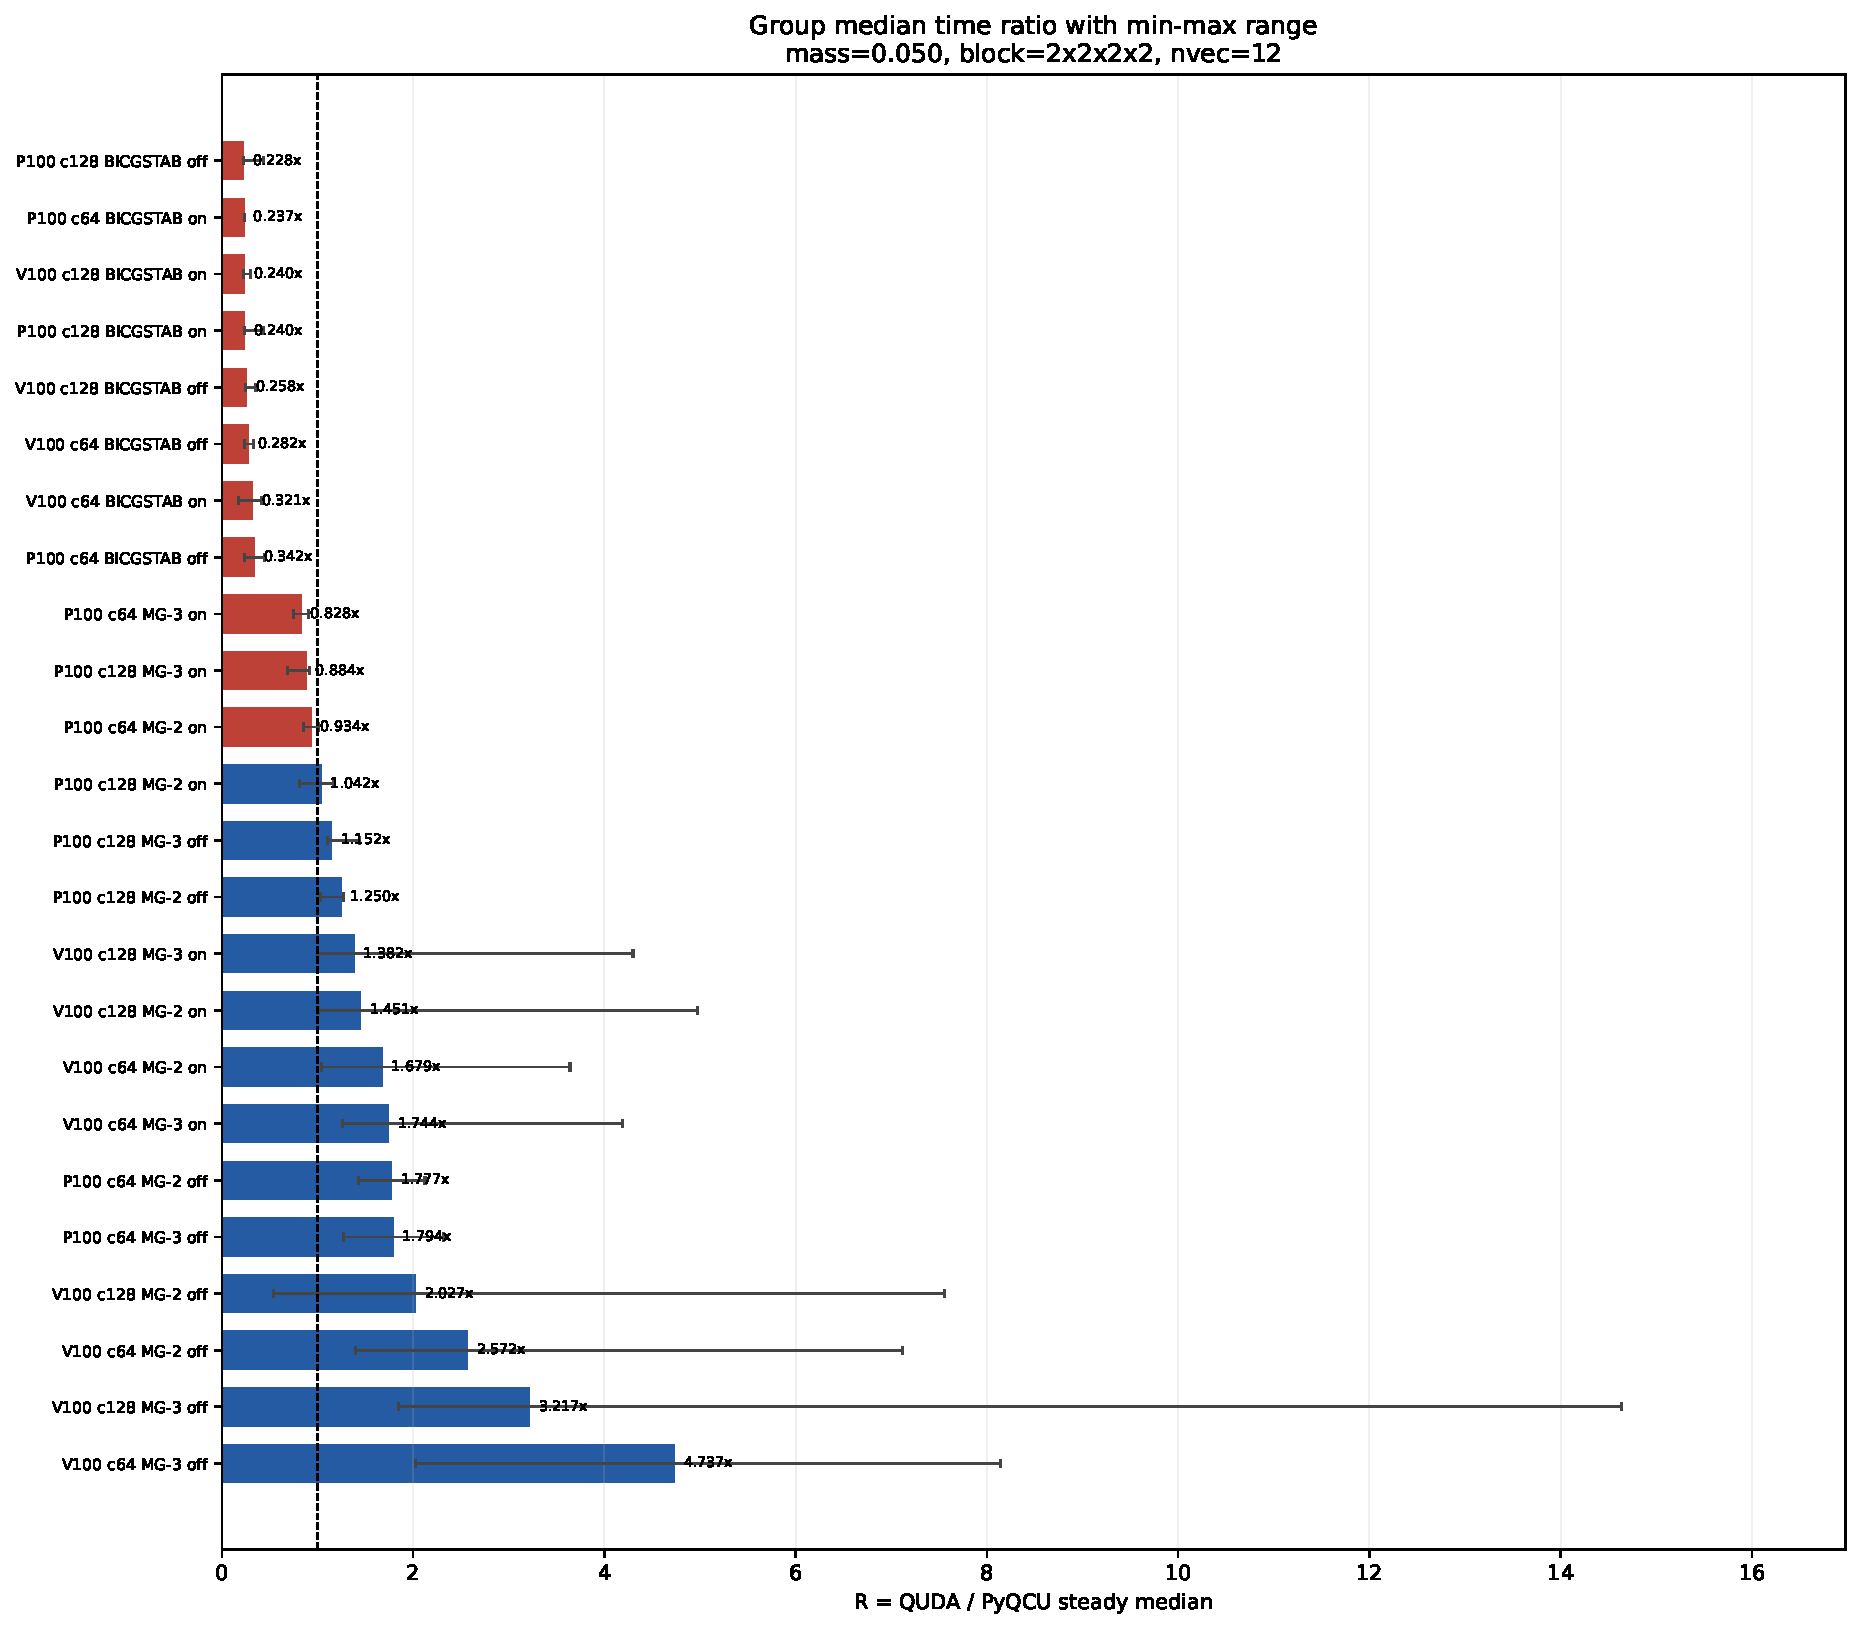
\includegraphics[width=0.98\linewidth,height=0.82\textheight,keepaspectratio]{mg_group_ratio_linear.pdf}
\caption{分组中位时间比与组内 min--max。正式性能只看 trace-off；
BiCGStab 组用于限定结论边界。}
\label{fig:group-ratio}
\end{figure}

\section{PyQCU Strict-MG 的实际路径}

\subsection{算法组合}

PyQCU test27 生产路径不是“CUDA dslash 加速的 Python MG”这一笼统说法，
而是以下明确组合：

\begin{figure}[htbp]
\centering
\begin{tikzpicture}[node distance=5mm and 5mm,scale=0.92,transform shape]
\node[pybox,text width=2.85cm] (rhs) {full RHS\\$[2,4,3,X,Y,Z,$\\$T/2]$};
\node[pybox,right=of rhs,text width=2.55cm] (prepare) {fine prepare\\归一化 odd MATPC};
\node[pybox,right=of prepare,text width=2.7cm] (outer) {right-FGMRES\\restart 16};
\node[pybox,right=of outer,text width=2.55cm] (mr1) {fine MR\\$\nu_{\rm pre}=1$};
\node[pybox,right=of mr1,text width=2.7cm] (restrict) {parity restriction\\$\to$ full coarse};
\node[pybox,below=of restrict,text width=2.7cm] (vcycle) {recursive V-cycle\\每层 MR};
\node[pybox,left=of vcycle,text width=2.55cm] (coarse) {coarsest fused\\cooperative BiCGStab};
\node[pybox,left=of coarse,text width=2.7cm] (prolong) {parity prolongation\\$\to$ fine correction};
\node[pybox,left=of prolong,text width=2.55cm] (mr2) {fine MR\\$\nu_{\rm post}=1$};
\node[pybox,left=of mr2,text width=2.55cm] (refresh) {true-residual\\refresh};
\draw[dataflow] (rhs)--(prepare);
\draw[dataflow] (prepare)--(outer);
\draw[dataflow] (outer)--(mr1);
\draw[dataflow] (mr1)--(restrict);
\draw[dataflow] (restrict)--(vcycle);
\draw[dataflow] (vcycle)--(coarse);
\draw[dataflow] (coarse)--(prolong);
\draw[dataflow] (prolong)--(mr2);
\draw[dataflow] (mr2)--(refresh);
\draw[dataflow] (refresh)--(outer);
\end{tikzpicture}
\caption{PyQCU test27 Strict-MG 的算法流水。蓝色框是实现路径，箭头表示
数据依赖；每个 restart 均回到同一个持久 hierarchy。}
\label{fig:pyqcu-flow}
\end{figure}

\begin{itemize}[leftmargin=2em]
  \item \confirmed{} 外层是 restarted right-preconditioned FGMRES。
        Cython 入口明确接收 \path{restart/max_iter/tolerance/nu_pre/nu_post}
        和固定 workspace 预算，C++ 保存 flexible preconditioned basis
        $Z$，再对 $AZ$ 做 Arnoldi。
  \item \confirmed{} 预条件器为 fine MR、parity restriction、递归 coarse
        V-cycle、parity prolongation、fine MR。非最粗层重复该结构；最粗层
        不递归，直接求 compact MATPC 系统。
  \item \confirmed{} 最粗层在单 rank 且 cooperative launch 可用时使用
        单个 fused cooperative BiCGStab kernel；多 rank 回退 host-scalar
        BiCGStab，因为 fused kernel 不包含 MPI collective。
  \item \confirmed{} coarse Galerkin 对象是
        $D_{c}=R(X_f^{-1}D_f)P$。运行时保存 $X$、$X^{-1}$、
        forward/backward $\widehat Y$ 和 transfer $V$，默认释放 raw $Y$。
  \item \confirmed{} test27 的 block 为 $(2,2,2,2)$，coarse spin 2，
        coarse dof 24，$\nu_{\rm pre}=\nu_{\rm post}=1$，coarse maxiter 200，
        restart 16。
\end{itemize}

\source{pyqcu/cuda/qcu/qcu.pyx:528-675;
pyqcu/cuda/_strict_multigrid.py:90-334;
cpp/cuda/qcu/src/apply_multigrid_strict.cu:4017-4053,4144-4298,4375-4685}

\subsection{数据结构}

Strict 路径把 fine full field、fine compact parity、coarse full field 和
blocked transfer 分成四类对象，ABI 与 kernel 一起固定：

\begin{table}[htbp]
\centering
\caption{PyQCU Strict-MG 的关键张量布局}
\footnotesize
\begin{tabularx}{\textwidth}{@{}L{0.31\textwidth}L{0.31\textwidth}Y@{}}
\toprule
对象 & 布局 & 物理/工程含义 \\
\midrule
full solution/RHS & \code{[2,4,3,X,Y,Z,T/2]} &
parity-split full field；目标 parity 是待求 MATPC 解，另一 parity 用于重构 \\
compact parity vector & \code{[12,X,Y,Z,T/2]} &
单 parity 上的 spin--color 12 dof；FGMRES 的 fine arena 使用此尺寸 \\
gauge/clover & \code{[2,3,3,4,...]}、
\code{[4,3,4,3,...]} &
输入 cache 即为 parity-split 连续 CUDA 张量，避免求解阶段重新切块 \\
coarse runtime links & \code{[2,4,E,E,X,Y,Z,T]} &
第一轴 forward/backward，第二轴方向；$E=24$ 是 coarse spin--color dof \\
coarse onsite pair & \code{[2,E,E,X,Y,Z,T]} &
$(X,X^{-1})$；coarse dslash 以 onsite + nearest-neighbour links 作用 \\
blocked transfer & \code{[E,e,Xc,bx,Yc,by,Zc,bz,Tc,bt]} &
10 维 blocked V；C++ restriction/prolongation 直接按该布局发散 \\
\bottomrule
\end{tabularx}
\end{table}

\source{pyqcu/cuda/qcu/qcu.pyx:180,277,330,418,528-598;
cpp/cuda/qcu/src/apply_multigrid_strict.cu:1499-1590,2926-3015}

\subsection{并行、通信与同步}

\begin{table}[htbp]
\centering
\caption{PyQCU Strict-MG 的并行执行模型}
\small
\begin{tabularx}{\textwidth}{@{}L{0.22\textwidth}Y@{}}
\toprule
维度 & test27 实际实现 \\
\midrule
rank 拓扑 & process grid 必须与 \code{MPI_COMM_WORLD} 一致；各层沿用同一
grid；local extent 必须偶数、与 block 对齐，aggregate 不跨 rank \\
设备映射 & 每个 rank 一张 GPU；V100 为 1 rank，P100 为 2 rank
$[2,1,1,1]$。同进程 N 线程 × N 卡的 \code{MultiGpuMultigrid}
不是 test27 的生产求解路径 \\
线程分配 & 核心 kernel 以 256 线程块为主；粗层 hopping 使用 256 线程
固定块；grid size 按 local/coarse volume 向上取整 \\
CUDA 流 & 每个 \code{LatticeSet} 有私有非阻塞 stream；粗层 halo 使用
独立 exchange stream 和 CUDA event，计算与通信可在 c64 路径重叠 \\
粗层通信 & 32 个方向 wire slot；向量 halo 走非阻塞
\code{MPI_Irecv/Isend}，local/remote-forward 分区；
backward link halo 逐维交换并可缓存 \\
c128 限制 & 分布式 c128 默认关闭 overlap，只有显式
\code{PYQCU_STRICT_OVERLAP_C128=1} 才启用；这是为保护 BiCGStab
轨迹和结果一致性而设的保守边界 \\
全局归约 & 多 rank dot 使用 \code{MPI_Allreduce}；单 rank 直接返回 local；
最粗 fused BiCGStab 只在单 rank 无 collective 场景启用 \\
\bottomrule
\end{tabularx}
\end{table}

\source{pyqcu/cuda/_strict_mpi.py:226-370,774-895;
cpp/cuda/qcu/src/apply_multigrid_strict.cu:1690-1929,2485-2545,
2607-2701,2953-3247,3617-3650}

\subsection{内存、cache 与生命周期}

\begin{itemize}[leftmargin=2em]
  \item \confirmed{} FGMRES 使用单一持久 arena，大小
        \begin{equation}
          B_{\rm fused}=(2m+5)B_f+2B_c,
        \end{equation}
        其中 $m$ 是 restart，$B_f$ 是一个 compact fine vector 字节数，
        $B_c$ 是一个 full first-coarse vector 字节数。Python 侧在 512 MiB
        默认预算内缩短 restart，并核对 C++ 返回的
        \code{allocated_bytes}，防止账本漂移。
  \item \confirmed{} 非最粗层持久保存 compact rhs/x、子层 full rhs、
        halo buffer 和 reduction scratch；同一 geometry/restart 下复用，
        不同 restart 才释放重配。
  \item \confirmed{} runtime 不持有 raw $Y$。在 c64 $16^4$ MG-3 样本中，
        cache 报告约 370.4 MB 的 V/Yhat/onsite resident assets，
        fused workspace 约 118.0 MB；raw-link 节省量约 160.4 MB。
  \item \confirmed{} HDF5 v2 strict cache 保存 fine blocked V、每层
        Yhat/onsite 和递归 V，校验 identity/shape/dtype/SHA256 后装载；
        test27 setup 使用 runtime cache restore，而非每次重建。
  \item \confirmed{} 关闭顺序是 StrictEnd、解绑 tensor/\code{set_ptrs}、
        applyEndQcu；setup hierarchy 在 runtime 绑定后可 seal，避免 Python
        与 C++ 同时保留两份 full setup 资产。
\end{itemize}

\source{pyqcu/cuda/_strict_multigrid.py:133-265,339-455;
pyqcu/cuda/_strict_cache.py:1-80,900-1030;
cpp/cuda/qcu/src/apply_multigrid_strict.cu:2953-3247,3315-3385}

\section{QUDA 1.1.0 的实际路径}

\subsection{算法组合}

test27 的 QUDA 侧是 native PyQUDA + QUDA 1.1.0 组合，不是 PyQCU 自己
扮演“QUDA 算法”的参考类。实际参数由 benchmark 显式设置并回读校验：

\begin{figure}[htbp]
\centering
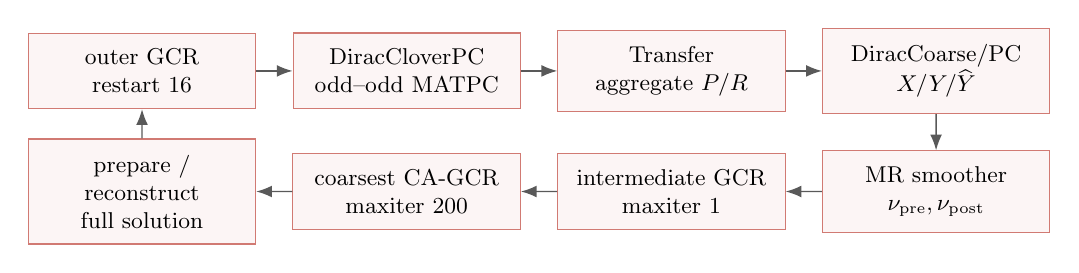
\begin{tikzpicture}[node distance=5mm and 5mm,scale=0.92,transform shape]
\node[qbox,text width=2.7cm] (outer) {outer GCR\\restart 16};
\node[qbox,right=of outer,text width=2.7cm] (clover) {DiracCloverPC\\odd--odd MATPC};
\node[qbox,right=of clover,text width=2.7cm] (transfer) {Transfer\\aggregate $P/R$};
\node[qbox,right=of transfer,text width=2.7cm] (coarse) {DiracCoarse/PC\\$X/Y/\widehat Y$};
\node[qbox,below=of coarse,text width=2.7cm] (smooth) {MR smoother\\$\nu_{\rm pre},\nu_{\rm post}$};
\node[qbox,left=of smooth,text width=2.7cm] (mid) {intermediate GCR\\maxiter 1};
\node[qbox,left=of mid,text width=2.7cm] (bottom) {coarsest CA-GCR\\maxiter 200};
\node[qbox,left=of bottom,text width=2.7cm] (recon) {prepare /\\reconstruct\\full solution};
\draw[dataflow] (outer)--(clover);
\draw[dataflow] (clover)--(transfer);
\draw[dataflow] (transfer)--(coarse);
\draw[dataflow] (coarse)--(smooth);
\draw[dataflow] (smooth)--(mid);
\draw[dataflow] (mid)--(bottom);
\draw[dataflow] (bottom)--(recon);
\draw[dataflow] (recon)--(outer);
\end{tikzpicture}
\caption{QUDA test27 的算法流水。红色框是 native QUDA 对象；
中间层 coarse solver 的 maxiter 为 1，最粗层为 CA-GCR。}
\label{fig:quda-flow}
\end{figure}

\begin{itemize}[leftmargin=2em]
  \item \confirmed{} 外层为 \code{QUDA_GCR_INVERTER}，
        \code{gcrNkrylov=16}，target 为
        \code{QUDA_MATPC_ODD_ODD}，实际求解路径是
        \code{QUDA_DIRECT_PC_SOLVE}。
  \item \confirmed{} smoother 各层均为 \code{QUDA_MR_INVERTER}，
        tolerance 0，$\nu_{\rm pre}=\nu_{\rm post}=1$。
  \item \confirmed{} 非最粗层 coarse solver 为 QUDA GCR 且 maxiter 1；
        最粗层为 QUDA CA-GCR，maxiter 200，tol 与 shared
        coarse tolerance 一致。
  \item \confirmed{} test27 显式将 setup、dslash、transfer 的
        \code{*_use_mma} 全部设为 false。因此该结果不是 QUDA
        Tensor-Core/MMA coarse path 的性能上限。
  \item \confirmed{} V100 运行使用 WSL2 patched QUDA 构建；
        provenance 明确记录 \code{DEV87_REDUCE_SYNC} 平台限制。
\end{itemize}

\source{pyqcu/testing/qcu/strict/quda_comparison/bench_strict_vs_quda.py:1623-1688,
4317-4457,4700-4816;
refer/git-rep/quda/lib/inv_gcr_quda.cpp:107-196;
refer/git-rep/quda/lib/multigrid.cpp:274-338,565-668,1175-1322}

\subsection{数据结构}

QUDA 以通用 field 类而不是 PyQCU 的固定显式 ABI 为中心：

\begin{table}[htbp]
\centering
\caption{QUDA 1.1.0 的关键对象}
\small
\begin{tabularx}{\textwidth}{@{}L{0.27\textwidth}L{0.30\textwidth}Y@{}}
\toprule
对象 & 关键字段/布局 & 作用 \\
\midrule
\code{ColorSpinorField} & \code{nVec}、\code{fieldOrder}、
\code{siteSubset}、ghost/pad & 普通向量、MG basis 和 vectorized
transfer；ghost zone 与字段一起管理 \\
\code{Transfer} & \code{B}、\code{V}、fine/coarse map、spin map &
null vectors、aggregate 映射、block orthogonalization 与 $P/R$ \\
\code{DiracCoarse} & coarse $X/Y$、\code{QUDA_COARSE_LINKS}、
bi-directional ghost & Galerkin 粗算子与 nearest-neighbour coarse dslash \\
\code{DiracCoarsePC} & $X^{-1}$、$\widehat Y$、MATPC prepare/reconstruct &
预条件粗算子；最粗层和 coarse smoother 可直接使用 \\
\code{QudaMultigridParam} & \code{geo_block_size}、\code{n_vec}、
\code{precision_null}、smoother/coarse solver、MMA flags &
一个公开的结构化配置面，表达比 test27 当前协议更多的组合 \\
\bottomrule
\end{tabularx}
\end{table}

\source{refer/git-rep/quda/include/color_spinor_field.h:103-211,270-360,468-695;
refer/git-rep/quda/lib/transfer.cpp:100-163,200-317;
refer/git-rep/quda/lib/dirac_coarse.cpp:121-297,351-430;
refer/git-rep/quda/include/quda.h:629-836}

\subsection{并行、通信与同步}

\begin{itemize}[leftmargin=2em]
  \item \confirmed{} test27 通过 QMP/PyQUDA 进入 native QUDA；
        QMP 提供 rank、消息句柄、非阻塞 start/wait/query 和 collective。
  \item \confirmed{} \code{ColorSpinorField::exchange} 会按 partitioned
        dimensions 声明 forward/backward send/receive，先
        \code{comm_start} 再 \code{comm_wait}，GPU field 默认经过聚合的
        pinned host staging，减少零散 D2H/H2D copy。
  \item \confirmed{} test27 的 QUDA 构建关闭 NVSHMEM，coarse dslash 因此
        不经过 SHMEM overlap 分支；运行时创建 9 条 CUDART stream，
        coarse halo 使用按方向编号的高优先级 stream，compute 走默认
        stream。
  \item \confirmed{} coarse fields 使用 native gauge order 和双向 ghost；
        \code{Y/X/Yhat/Xinv} 都存在 ghost padding，分配时按最大 face
        预留空间。
  \item \confirmed{} QUDA 的 MG solver factory 能配置不同精度、不同
        location、smoother/coarse solver 和 cycle type；这是宽度优势，
        但 test27 只实例化了 odd--odd MATPC、MR、GCR/CA-GCR 的固定组合。
\end{itemize}

\source{refer/git-rep/quda/lib/communicator_qmp.cpp:175-303;
refer/git-rep/quda/lib/color_spinor_field.cpp:540-667;
refer/git-rep/quda/lib/targets/cuda/device.cpp:281-330;
refer/git-rep/quda/lib/dslash_coarse.hpp:468-525;
data/quda-qio-build/attempt2/CMakeCache.txt:1127;
refer/git-rep/quda/lib/dirac_coarse.cpp:121-223;
refer/git-rep/quda/lib/multigrid.cpp:274-430,565-668}

\subsection{内存、field cache 与部署接口}

\begin{itemize}[leftmargin=2em]
  \item \confirmed{} QUDA 以 \code{pool_device_malloc}、
        \code{pool_pinned_malloc} 和 FieldTmp cache 复用临时
        ColorSpinorField；适合多算法共享，但 PyQUDA 不暴露完整 native
        workspace 账本。
  \item \confirmed{} \code{GaugeField}/\code{ColorSpinorField} 自带
        location、field order、ghost、padding 和 lazy CPU/GPU copy；
        coarse asset 可以按需从 host 映到 device。
  \item \confirmed{} 公共接口是
        \code{newMultigridQuda/updateMultigridQuda/dumpMultigridQuda}
        加 \code{invertQuda}；配置面稳定，但多数运行期细节由 QUDA
        singleton、field cache、QMP communicator 和 autotuning 隐藏。
  \item \inferred{} test27 的 device-wide memory sampler 表明 QUDA
        的峰值通常更高，部分来自 ghost padding、native coarse fields 和
        field pool；由于 sampler 可能包含其他进程，不能把这个差值直接
        当作泄漏或算法内存下界。
\end{itemize}

\source{refer/git-rep/quda/include/malloc_quda.h:165-174;
refer/git-rep/quda/include/field_cache.h:44-124;
refer/git-rep/quda/include/color_spinor_field.h:103-211,270-360;
refer/git-rep/quda/include/quda.h:1230-1289}

\section{逐维比较：两种设计的优缺点}

\begin{landscape}
\begin{xltabular}{0.97\linewidth}{@{}L{0.13\linewidth}L{0.23\linewidth}L{0.23\linewidth}L{0.23\linewidth}@{}}
\caption{MultiGrid 设计的跨维度比较。表中“优势”是相对该项，不是全局胜负。}\label{tab:cross-dimension}\\
\toprule
维度 & PyQCU Strict-MG & QUDA 1.1.0 & 评价与边界 \\
\midrule
\endfirsthead
\toprule
维度 & PyQCU Strict-MG & QUDA 1.1.0 & 评价与边界 \\
\midrule
\endhead
算法组合 &
right-FGMRES + fine/coarse MR + recursive V-cycle + coarsest fused
BiCGStab；只实现 Wilson--Clover strict 路径 &
可变 solver factory；test27 实际为 outer GCR + MR + intermediate GCR(1)
+ coarsest CA-GCR(200) &
\textbf{PyQCU 优势：} test27 的外层迭代普遍更少，算法与本问题更贴合。
\textbf{QUDA 优势：} 可选择 solver、精度、location 和 cycle，覆盖面更广。\\
\midrule
粗算子 &
$D_c=R(X_f^{-1}D_f)P$；runtime 只保留 $X,X^{-1},\widehat Y,V$；
nearest-neighbour stencil 是强约束 &
aggregate transfer + native \code{DiracCoarse/PC}; $X/Y/\widehat Y$
存储为带 ghost 的 GaugeField；支持逐层 location/精度 &
\textbf{PyQCU 优势：} 省去 raw $Y$，资产更小、ABI 更直接。
\textbf{QUDA 优势：} 通用粗算子、ghost、CPU/GPU lazy copy 与 MMA 路径成熟。\\
\midrule
数据结构 &
固定 C-order 张量 ABI；fine full/compact 与 coarse full 分离；
10-D blocked V &
\code{ColorSpinorField}/\code{GaugeField}，runtime 选择 field order、
ghost、nVec、site subset &
\textbf{PyQCU 优势：} 调试与字节账本透明。
\textbf{QUDA 优势：} 多算法、多精度和多 I/O 接口复用，工程覆盖更广。\\
\midrule
并行方案 &
MPI rank--GPU 一对一；每层同 process grid；32 向 coarse halo；
c64 向量 halo overlap，link/fine 通信仍含阻塞段 &
QMP 消息句柄、native field ghost/pad、peer-to-peer 和 autotuned
communication policy；分布式生产覆盖成熟 &
\textbf{PyQCU 优势：} 粗层 local/remote 分区使 c64 能重叠一部分通信。
\textbf{QUDA 优势：} 更成熟的多 rank、多 GPU 与硬件 backend 适配。\\
\midrule
同步策略 &
私有 compute stream；交换 stream + CUDA event；coarsest fused kernel
单 rank 无每迭代 host round-trip & GCR/Coarse 各阶段独立 sync policy；
QMP start/wait；GPU ghost 经聚合 staging；kernel 与调优缓存分隔 &
\textbf{PyQCU 优势：} 单 rank 粗层递推融合，减少 launch/sync 次数。
\textbf{QUDA 优势：} sync policy 与通信栈跨配置成熟，不只针对一个
odd--odd c64 样本。\\
\midrule
内存管理 &
固定 fused arena 公式；512 MiB 默认预算；HDF5 strict cache；
runtime-owned bytes 可账本化 &
field pool + pinned buffer pool + FieldTmp cache；ghost padding；
lazy CPU/GPU；native workspace 不完整暴露 &
\textbf{PyQCU 优势：} 可预测、可验证、test27 观测峰值较低。
\textbf{QUDA 优势：} 配置选择和生命周期抽象更通用，但内存上界更难
由 Python 侧完整核算。\\
\midrule
调用接口 &
int32[58] params + float[7] argv + int64[100] \code{set_ptrs}；必须显式管理
init/end、set index、cache 和 workspace &
\code{QudaMultigridParam} + \code{invertQuda}；
PyQUDA/PyTorch 传 field；有 update/dump 接口 &
\textbf{PyQCU 优势：} 固定 ABI 方便专用 kernel 和精确 provenance。
\textbf{QUDA 优势：} 面向使用者更稳定、组合更丰富、部署生态更完整。\\
\midrule
能力边界 &
最多 5 层；fine dof 固定 12；要求偶数 extent/最近邻 strict stencil；
逐层 mixed precision 当前 fail-closed &
支持更多 Dirac/transfer/coarse 组合与硬件 backend；但参数组合也更容易
产生非可比配置 &
\textbf{结论：} PyQCU 是窄而深的专用实现；QUDA 是宽而成熟的生产框架。\\
\bottomrule
\end{xltabular}
\end{landscape}

\section{test27 性能分解：优势从哪里来}

\subsection{迭代数与单迭代成本的乘积分解}

对每个精确 MG 单元定义
\begin{equation}
  R=\frac{t_Q}{t_P}
    =\underbrace{\frac{N_Q}{N_P}}_{\text{迭代比}}
     \underbrace{
       \frac{t_Q/N_Q}{t_P/N_P}
     }_{\text{单外层迭代成本比}},
\end{equation}
其中 $P=\mathrm{PyQCU}$，$Q=\mathrm{QUDA}$。该分解不改变任何原始时间，
只是把公开的 steady time 与 outer iteration 两个字段相乘重排。

\begin{table}[htbp]
\centering
\caption{trace-off MG 的代表性比值分解}
\small
\begin{tabularx}{\textwidth}{@{}L{0.28\textwidth}rrrY@{}}
\toprule
单元 & $N_Q/N_P$ & 单迭代成本比 & $R$ & 解释 \\
\midrule
V100 c64 $16^4$ MG-3 & 1.903 & 2.489 & 4.737 &
PyQCU 少约 47\% 外层迭代，且 QUDA 单迭代更贵 \\
V100 c128 $8^3\times16$ MG-3 & 3.214 & 4.553 & 14.634 &
小格上 setup/launch 与轨迹差异被放大 \\
V100 c64 $16\times32\times32\times48$ MG-2 & 3.364 & 0.416 &
1.400 & PyQCU 外层更少，但单迭代更贵，仍净胜 \\
V100 c128 $16\times16\times32\times32$ MG-2 & 2.073 & 0.261 &
0.540 & 唯一 trace-off MG 负例；迭代优势不足以抵消单迭代成本 \\
\bottomrule
\end{tabularx}
\end{table}

\begin{figure}[htbp]
\centering
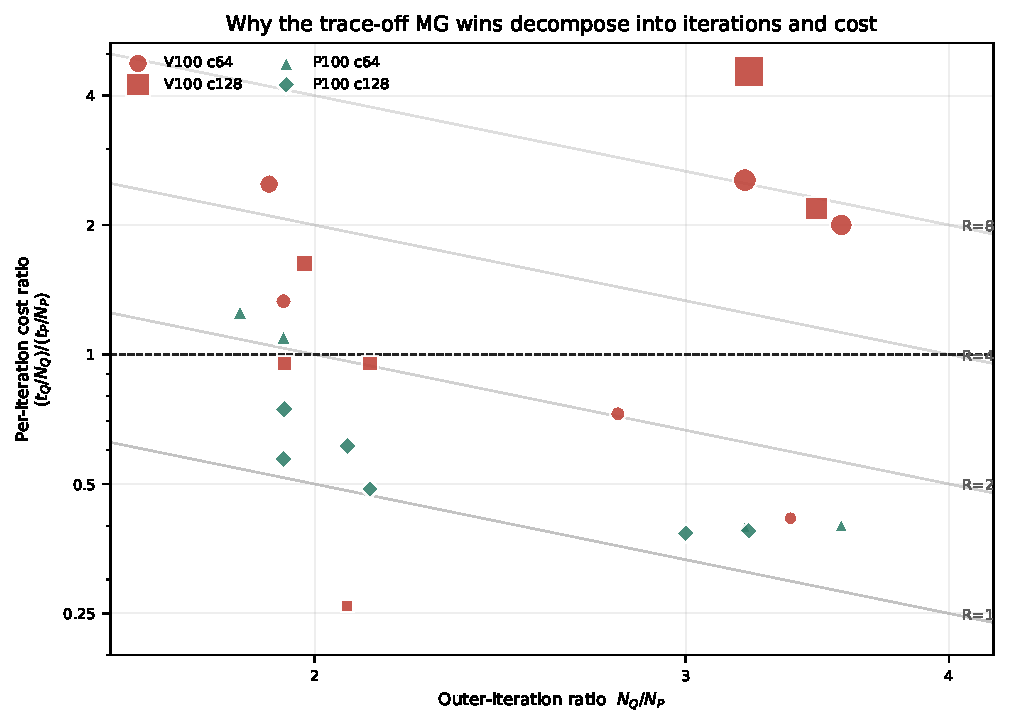
\includegraphics[width=0.96\linewidth,height=0.73\textheight,keepaspectratio]{mg_ratio_decomposition_20261002.pdf}
\caption{22 个 trace-off MG 单元的迭代/单迭代成本分解。点越靠右表示
PyQCU 外层迭代越少；点越靠上表示 QUDA 单迭代越贵；等 $R$ 线为双曲线。
点大小随 $R$ 增加。}
\label{fig:ratio-decomposition}
\end{figure}

\begin{conclusionbox}
\textbf{定量主因。} trace-off MG 的迭代比中位数为 2.125，而单迭代成本比
中位数为 0.8498。44 个 MG 单元全部由 PyQCU 使用更少外层迭代。这个结果是
“算法轨迹 + 调度实现”的联合结果，不能单独归因成某个 CUDA kernel。
\end{conclusionbox}

\subsection{设备、精度、格点与 trace}

\begin{figure}[htbp]
\centering
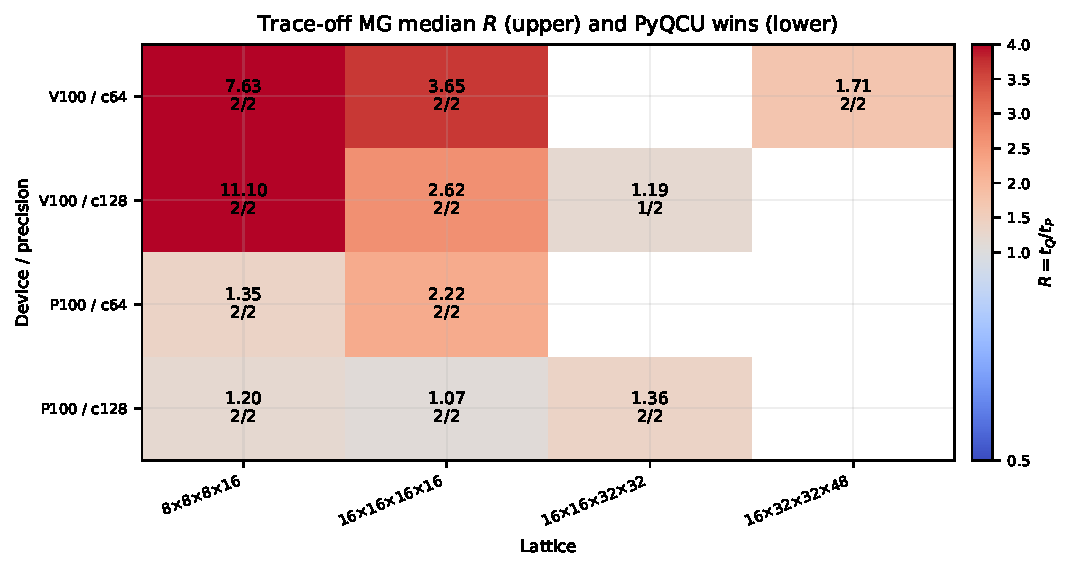
\includegraphics[width=0.96\linewidth,height=0.68\textheight,keepaspectratio]{mg_win_matrix_20261002.pdf}
\caption{trace-off MG 的格点矩阵。单元格上行为 MG-2/MG-3 的中位 $R$，
下行为 PyQCU 胜点数；空白表示该设备/精度没有对应格点。}
\label{fig:win-matrix}
\end{figure}

\begin{figure}[p]
\centering
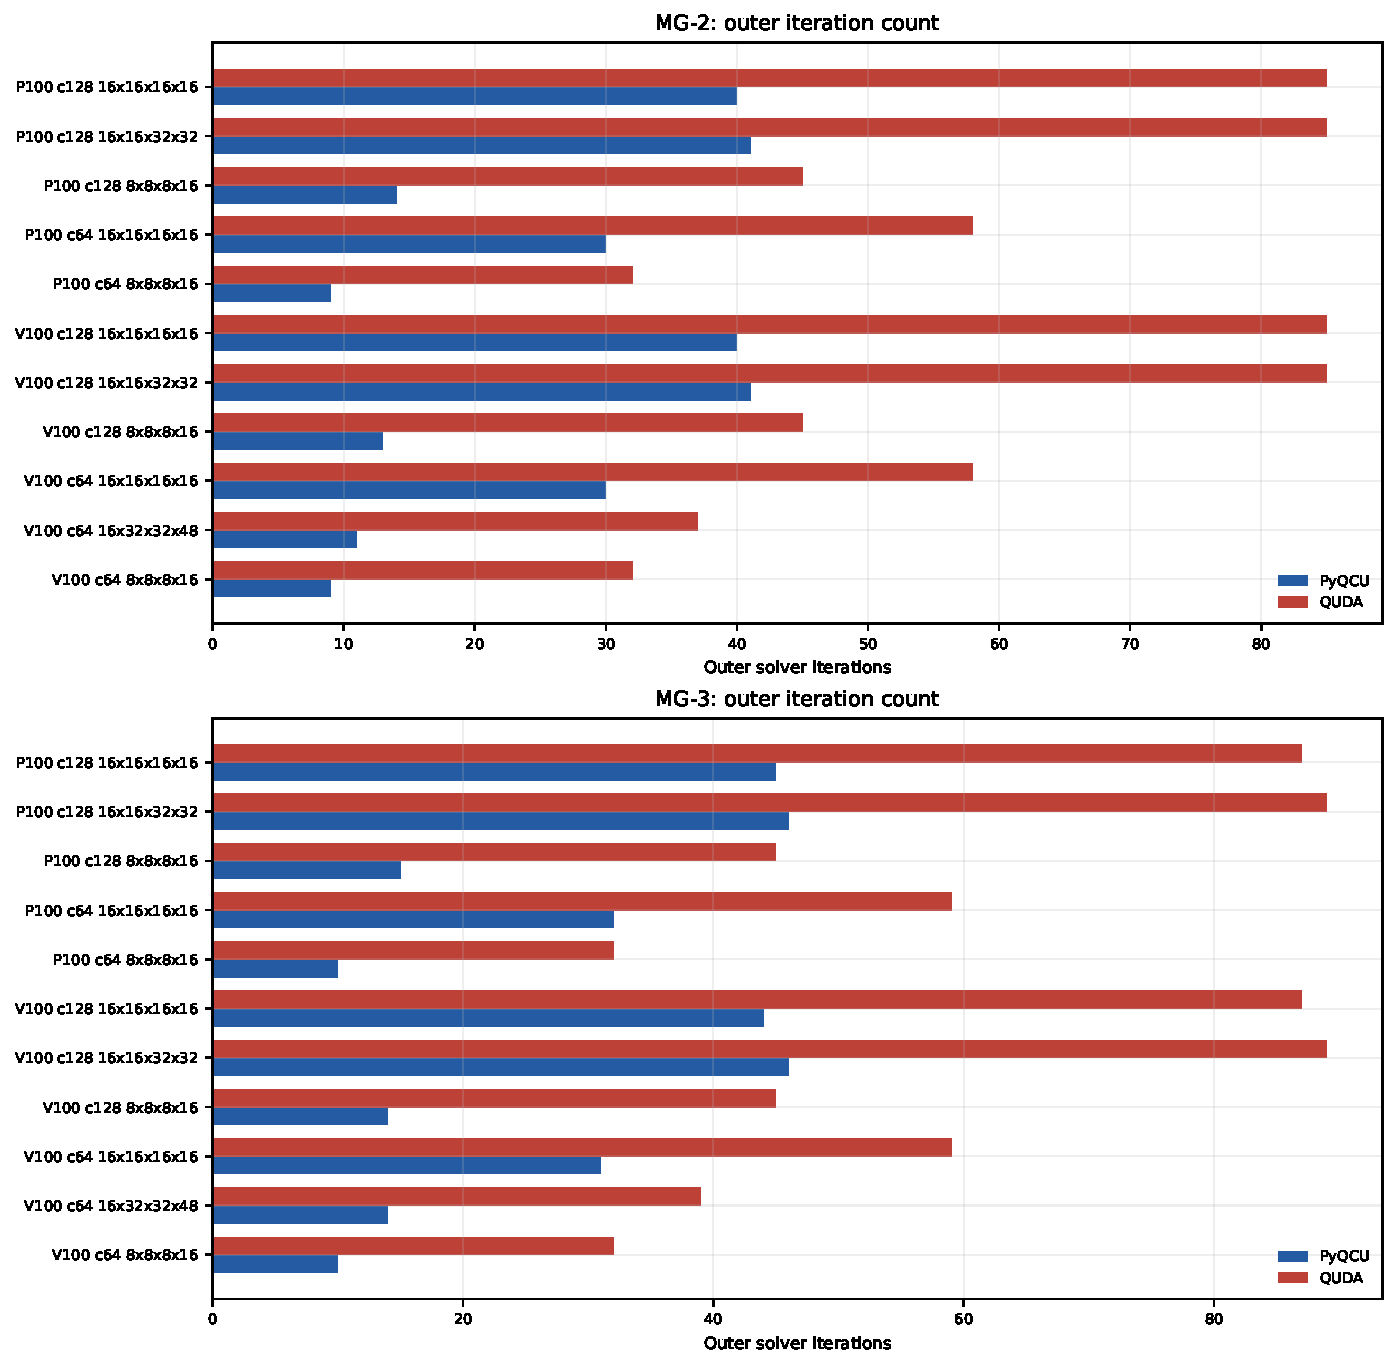
\includegraphics[width=0.96\linewidth,height=0.82\textheight,keepaspectratio]{mg_outer_iterations_20261002.pdf}
\caption{trace-off MG 的外层迭代逐单元对照。两面板分别对应 MG-2 和 MG-3；
这是“为什么更快”的最强单变量证据之一。}
\label{fig:outer-iterations}
\end{figure}

\begin{table}[htbp]
\centering
\caption{按设备和精度的 MG 胜负}
\small
\begin{tabular}{@{}llrrrr@{}}
\toprule
设备 & 精度 & 单元数 & 中位 $R$ & PyQCU 胜 & QUDA 胜 \\
\midrule
V100 & c64 & 10 & 2.2186 & 10 & 0 \\
V100 & c128 & 12 & 1.3581 & 11 & 1 \\
P100 & c64 & 10 & 1.2742 & 10 & 0 \\
P100 & c128 & 12 & 1.1084 & 11 & 1 \\
\bottomrule
\end{tabular}
\end{table}

上述数据只使用 trace-off。trace-on 的中位 $R$ 从 1.9358 降到 1.0404，
说明诊断同步会显著扰动性能；所有正式倍率均不读取 trace-on。

\subsection{setup、阶段与最粗层}

setup 不计入 solve-only 时间比。下表只说明运行准备成本，
\code{runtime cache restore} 与 QUDA native setup 不是同一种计算。

\begin{figure}[htbp]
\centering
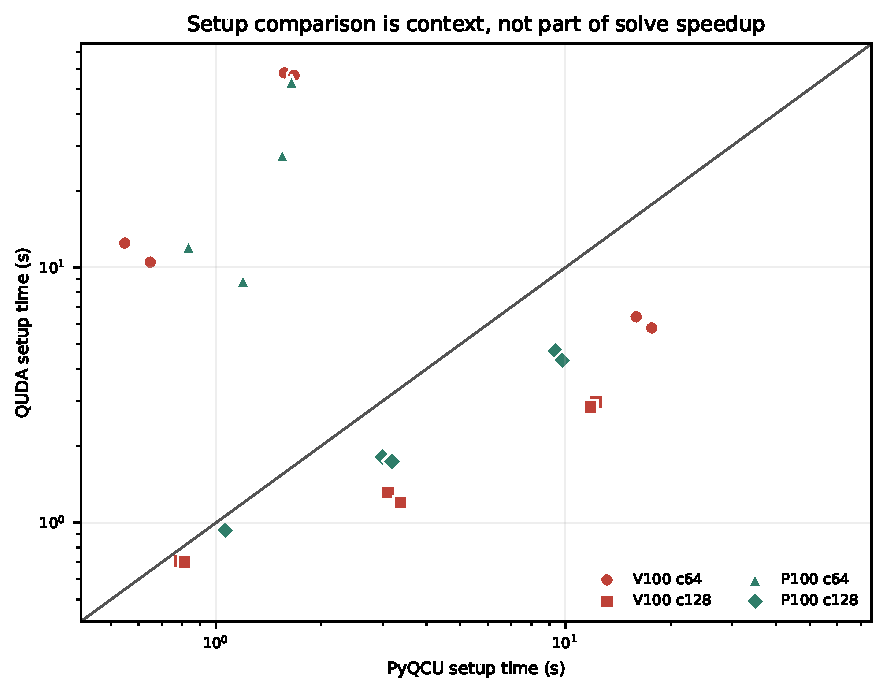
\includegraphics[width=0.88\linewidth,height=0.62\textheight,keepaspectratio]{mg_setup_context_20261002.pdf}
\caption{trace-off MG 的 setup 上下文。点在对角线上方表示 QUDA setup
更贵；由于 PyQCU 使用 cache restore，图中差异不得混入 solve speedup。}
\label{fig:setup-context}
\end{figure}

\begin{table}[htbp]
\centering
\caption{最粗层 solve 的绝对中位耗时；QUDA 的最后有效层已显式取回}
\small
\begin{tabular}{@{}llrrrr@{}}
\toprule
设备 & 精度/层数 & $n$ & PyQCU s & QUDA s & $R=Q/P$ \\
\midrule
P100 & c128 / MG-2 & 3 & 41.416 & 23.296 & 0.5625 \\
P100 & c128 / MG-3 & 3 & 14.781 & 9.799 & 0.6629 \\
P100 & c64 / MG-2 & 2 & 8.519 & 5.758 & 0.6758 \\
P100 & c64 / MG-3 & 2 & 5.148 & 2.201 & 0.4275 \\
V100 & c128 / MG-2 & 3 & 5.603 & 4.137 & 0.7384 \\
V100 & c128 / MG-3 & 3 & 0.867 & 1.607 & 1.8538 \\
V100 & c64 / MG-2 & 3 & 1.420 & 1.124 & 0.7917 \\
V100 & c64 / MG-3 & 3 & 0.438 & 0.977 & 2.2279 \\
\bottomrule
\end{tabular}
\end{table}

\source{data/report_multigrid_comprehensive_20261001/report/coarsest_times.csv;
data/report_multigrid_comprehensive_20261001/report/stage_component_medians.csv}

\begin{center}
\begin{tabularx}{\textwidth}{@{}L{0.30\textwidth}Y@{}}
\toprule
现象 & 解释边界 \\
\midrule
V100/c64 MG-3 最粗层 PyQCU 约快 2.23$\times$ &
单 rank fused cooperative BiCGStab 与 QUDA CA-GCR 的直接差异 \\
P100/c128 MG-2/3 最粗层 PyQCU 慢 1.5--1.8$\times$ &
多 rank 时 PyQCU fused kernel 被禁用，host-scalar fallback 的成本更高 \\
PyQCU 阶段 tracing 的 \code{other} 占比较高 &
两侧阶段边界并非完全同构；只能解释粗层量级，不能把每个 percentage
当作同分母物理成本 \\
\bottomrule
\end{tabularx}
\end{center}

\subsection{显存}

下表使用 \code{steady_sampler_peak_bytes}，即不计时 post-timing
device-wide \code{cudaMemGetInfo} 采样，可能包含测试进程之外的同设备
分配。它用于门限与趋势，不声明为进程独占峰值。

\begin{table}[htbp]
\centering
\caption{steady device-wide 显存汇总（GiB）}
\small
\begin{tabular}{@{}lrrrr@{}}
\toprule
侧 & 样本 & P50 & P95 & max \\
\midrule
PyQCU & 66 & 2.615 & 11.224 & 11.628 \\
QUDA & 66 & 3.274 & 21.522 & 22.523 \\
\bottomrule
\end{tabular}
\end{table}

\begin{figure}[htbp]
\centering
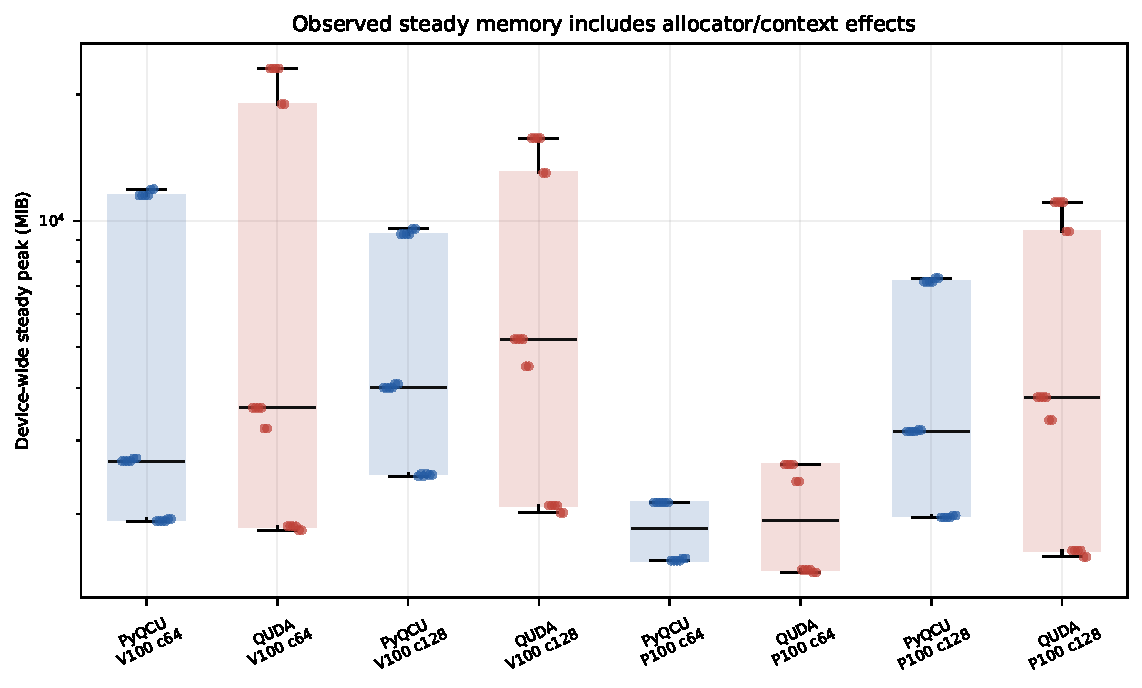
\includegraphics[width=0.96\linewidth,height=0.65\textheight,keepaspectratio]{mg_memory_distribution_20261002.pdf}
\caption{按设备/精度/侧分组的 steady memory 分布。箱线图显示中位与四分位，
散点为原始 side samples；纵轴为对数坐标。}
\label{fig:memory-distribution}
\end{figure}

\inferred{} 较低峰值有利于大格常驻与 cache 复用，这可能是 PyQCU 在大格
或 cache-warm 条件下的一个优势来源；但 test27 没有独立的“固定算法、
固定迭代数、仅改变分配器”实验，因此不能把显存下降直接等价为 solve
时间下降。

\section{客观分析：为什么 PyQCU 在 test27 超过 QUDA}

\subsection{可以确认的原因}

\begin{enumerate}[leftmargin=2em]
  \item \textbf{外层迭代数更少。}
        \confirmed{} 44 个 MG 单元全部为 PyQCU outer iterations 更少；
        trace-off MG 的迭代比中位数为 2.125，部分大格达到 3.2--3.5。
        在相同 restart=16、相同 MATPC、相同零初值下，这是最直接的
        performance mechanism。
  \item \textbf{单 rank 粗层递推融合。}
        \confirmed{} PyQCU 在单 rank 把最粗层 BiCGStab 的 hopping、dot、
        recurrence 和 breakdown guard 合并到一个 cooperative kernel，
        避免每迭代的多次 kernel launch 与 host scalar round-trip。
        V100/c64 MG-3 最粗层中位时间 0.438 s，QUDA 为 0.977 s。
  \item \textbf{统一 FGMRES arena 减少了工作区碎片和管理开销。}
        \confirmed{} PyQCU 的 V/Z/b/r/w/x 与 coarse R/P field 在一个
        $(2m+5)B_f+2B_c$ arena 内，restart 和预算在 Python 边界即确定，
        C++ 不按 krylov vector 逐次扩张。
  \item \textbf{cu64 coarse path 的通信重叠。}
        \confirmed{} 分布式 c64 默认开启 vector halo overlap，local kernel
        只算本地和 remote-forward 基础项，远邻项在非阻塞交换后补算；
        这降低 P100 双 rank 的通信暴露。
  \item \textbf{runtime asset 更窄。}
        \confirmed{} PyQCU 只保留 $X,X^{-1},\widehat Y,V$，默认释放 raw
        $Y$；在 test27 的大多数样本中，device-wide peak 低于 QUDA。
\end{enumerate}

\subsection{只能作为推断的原因}

\begin{enumerate}[leftmargin=2em]
  \item \inferred{} 外层算法不是同一个数学迭代：PyQCU 使用 FGMRES，
        QUDA 使用 GCR；QUDA 中间层 coarse solver maxiter 为 1，最粗层
        CA-GCR 为 200。少迭代可能同时来自 Krylov 轨迹、preconditioner、
        coarse tolerance 和 smoother 组合，无法仅凭现有数据拆成单一
        kernel 贡献。
  \item \inferred{} V100/c64 的 2.2--4.7$\times$ 优势比 P100/c128
        更稳定，可能来自单 rank fused coarsest kernel、较少 MPI staging
        和更好 cache locality；但这些因素与设备、精度和 rank 数共同变化。
  \item \inferred{} memory peak 较低可能改善 L2/allocator 行为，
        但现有数据不足以证明它独立解释了 solve-time ratio。
\end{enumerate}

\subsection{不能确认或不能推广的部分}

\begin{enumerate}[leftmargin=2em]
  \item \unverified{} QUDA 在 test27 禁用 MMA；不能把本次结果写成
        PyQCU 对 QUDA 最强调优路径的普遍胜利。
  \item \unverified{} V100 QUDA 运行带 WSL2 \code{DEV87_REDUCE_SYNC}
        构建属性；该先验差异没有被本轮 on/off 消融隔离。
  \item \unverified{} BiCGStab 参考的计时边界、算法族和迭代数与 MG
        不同；22/22 QUDA 胜只能说明参考求解器更强，不能反推 coarse
        operator 的正确性或优劣。
  \item \unverified{} 当前精确样本主要是 1 rank V100 与 2 rank P100；
        多节点、高 rank、网络拓扑和 c128 overlap 的 scaling 不在本数据
        的可信外推范围内。
\end{enumerate}

\section{双方各自的优点与短板}

\begin{table}[htbp]
\centering
\caption{双方优势与短板的对象化总结}
\small
\begin{tabularx}{\textwidth}{@{}L{0.19\textwidth}Y Y@{}}
\toprule
维度 & PyQCU & QUDA 1.1.0 \\
\midrule
强项 &
窄路径深优化；固定 ABI；单 rank fused coarsest；显式内存预算；
test27 中更少 FGMRES 外层迭代；可追溯 cache 与源码贴近 &
solver/factory/精度/location 组合广；native field+ghost+QMP 成熟；
分布式、多 GPU、MMA、I/O 和硬件 backend 覆盖更完整；
BiCGStab 参考显著领先 \\
\midrule
短板 &
最多 5 层；12 dof Wilson--Clover 专用；最近邻 strict fail-closed；
多 rank coarsest 回退 host-scalar；fine dslash 通信仍阻塞；
用户接口偏底层，维护生命周期成本高 &
参数空间复杂；native workspace 不完整暴露；ghost/pool/native 分配
使显存上界较难归因；test27 的 disable-MMA 与 WSL2 patch 使结果
不代表其全部性能上限 \\
\bottomrule
\end{tabularx}
\end{table}

\section{后续优化方案}

\subsection{第一优先级：补足多 rank 粗层}

\begin{enumerate}[leftmargin=2em]
  \item 为多 rank coarsest solve 增加设备端 global reduction 与非阻塞
        coarse halo，使 fused cooperative kernel 不因缺少 collective
        盲目退化为 host-scalar 循环。
  \item 将 reduction、residual refresh 和 coarse link halo 纳入统一
        pipeline，目标是在 P100 两 rank 及更高 rank 保持 trace-off MG
        的真实残差门不变。
  \item 验收门：同一 input bundle、同一 restart，真残差 max
        $<5\times10^{-6}$，trace-off MG 中位 $R$ 在 P100 子集提高；
        不满足任一条件则不替换生产路径。
\end{enumerate}

\subsection{第二优先级：FGMRES/MR 的数值与调度联合调优}

\begin{enumerate}[leftmargin=2em]
  \item 建立 restart、smoother step、coarse tolerance 的三维自动搜索，
        但不能改变 test27 的正式协议后再宣称同一倍率。
  \item 研究 adaptive restart 和 spectrum-aware coarse tolerance；
        当前优势首先来自更少外层迭代，优化目标应明确为
        “减少总 V-cycle 数”而不是只压低单 kernel 时间。
  \item 对 c128 保留保守 overlap 默认；任何开启实验都必须同时记录
        BiCGStab trajectory、真残差和相同输入下的迭代分布。
\end{enumerate}

\subsection{第三优先级：把 setup 从 Python 批处理继续下沉}

\begin{enumerate}[leftmargin=2em]
  \item 将 colored Galerkin、block orthogonalization、$X^{-1}$ 和
        $\widehat Y$ 的剩余 Python/tensor 批处理收敛到专用 CUDA kernel。
  \item 对 cache miss 单独设置性能门；cache hit 只验证恢复、identity
        和内存账本，不再隐藏 setup 构建成本。
  \item 验收门：相同 lattice、精度和 block 下，cold setup 时间降低且
        cache 与运行时 resident asset 字节不变或更少。
\end{enumerate}

\subsection{第四优先级：通信与可移植性}

\begin{enumerate}[leftmargin=2em]
  \item 将 fine Wilson/Clover halo 从阻塞 \code{Sendrecv} 扩展到可组合的
        非阻塞路径，并优先覆盖 c128 与高 rank。
  \item 扩展 process-grid agglomeration、逐层 mixed precision、
        非 $12$ fine dof 和更一般 stencil 的 fail-closed 检查；
        在语义不可证明时继续拒绝，不把“能运行”当成“等价”。
  \item 建立 V100/P100/A100/H100 和 1/2/4/8 rank 的同一协议矩阵；
        报告必须包含算法组合、MMA 开关和通信 policy，避免跨配置混算。
\end{enumerate}

\subsection{第五优先级：用户接口与运行时治理}

\begin{enumerate}[leftmargin=2em]
  \item 保留底层 ABI，但在其上提供 “construct hierarchy / solve /
        update assets / close” 的高层 Python 对象，减少显式
        \code{_SET_INDEX_} 和 set pointer 误用。
  \item 将由同一机器可读 manifest 生成的 params/argv/\code{set_ptrs}
        跨语言常量作为唯一来源，持续检查
        \path{pyqcu/cuda/define.py} 与
        \path{cpp/cuda/qcu/include/define.h} 一致。
  \item 为 runtime cache、workspace 和 setup hierarchy 增加统一 memory
        ledger，区分 borrowed input、runtime-owned asset、fused workspace
        和 allocator reserve；避免把 device-wide 峰值当成进程独占值。
\end{enumerate}

\section{复现、验证与限制}

\subsection{数据重建}

\begin{verbatim}
python -B pyqcu/testing/qcu/strict/quda_comparison/\
plot_mg_architecture_report.py --check

python -m pytest -q pyqcu/testing/qcu/strict/quda_comparison/\
test_plot_mg_architecture_report.py
\end{verbatim}

生成器执行三类校验：

\begin{enumerate}[leftmargin=2em]
  \item 原始矩阵 66/66 combined、132/132 side、22/22/22 levels；
  \item 每个 side 的 1 cold / 2 warmup / 5 steady、config hash、
        input bundle 和真残差门；
  \item 新算出的 66 个 steady seconds 与 20261001 的 66 行派生表
        逐单元一致。
\end{enumerate}

\subsection{输出目录}

\begin{verbatim}
data/report_multigrid_comprehensive_20261002/report/
  unit_analysis.csv
  group_analysis.csv
  algorithm_profiles.csv
  summary.json
  source_hashes.json
  mg_ratio_decomposition_20261002.pdf
  mg_win_matrix_20261002.pdf
  mg_outer_iterations_20261002.pdf
  mg_setup_context_20261002.pdf
  mg_memory_distribution_20261002.pdf
\end{verbatim}

\subsection{已知限制}

\begin{itemize}[leftmargin=2em]
  \item test27 只有一个 P100 c64 大格请求触发容量替代；替代项不进入
        原大格公平倍率。
  \item QUDA 的 native workspace 未被 PyQUDA 完整暴露，显存比较以
        device-wide sampler 为主，不能声称进程独占峰值。
  \item PyQCU 的 trace-on 阶段定义与 QUDA 的阶段 boundary 不完全相同，
        只能做粗层量级和总 solve time 的可比分析。
  \item test27 没有做“同算法、同迭代数、只切换通信/allocator”的完整
        2×2 消融，因此本报告把 kernel、算法和调度贡献严格分级。
  \item test27 的 combined JSON 完整保存外层 invert 参数和 MG 参数，但
        \path{QudaMultigridParam::invert_param} 所指向的内部对象没有被
        独立序列化。未来重建应把该指针的目标字段也写入 provenance，
        消除内部 MATPC parity/solution type 仅靠构造关系的残余不确定性。
\end{itemize}

\section{源码证据索引}

\begin{landscape}
\begin{longtable}{@{}L{0.19\linewidth}L{0.34\linewidth}L{0.34\linewidth}@{}}
\caption{关键源码与数据证据索引}\label{tab:source-index}\\
\toprule
对象 & PyQCU & QUDA / 原始数据 \\
\midrule
\endfirsthead
\toprule
对象 & PyQCU & QUDA / 原始数据 \\
\midrule
\endhead
外层 FGMRES &
\path{cpp/cuda/qcu/src/apply_multigrid_strict.cu}:4144--4298；
\path{pyqcu/cuda/qcu/qcu.pyx}:528--675 &
\path{refer/git-rep/quda/lib/inv_gcr_quda.cpp}:107--196；
\path{refer/git-rep/quda/lib/multigrid.cpp}:565--668 \\
pre/post smoother &
\path{cpp/cuda/qcu/src/apply_multigrid_strict.cu}:3997--4075,4356--4380 &
\path{refer/git-rep/quda/lib/multigrid.cpp}:274--338,1209--1283 \\
V-cycle/coarsest &
\path{cpp/cuda/qcu/src/apply_multigrid_strict.cu}:4375--4685 &
\path{refer/git-rep/quda/lib/multigrid.cpp}:1175--1322；
\path{refer/git-rep/quda/include/multigrid.h}:128--304 \\
$P/R$、$X/Y/\widehat Y$ &
\path{pyqcu/solver/_quda_multigrid.py}:349--597,1071--1558；
\path{pyqcu/tools/_strict_galerkin.py}:1--80,480--720 &
\path{refer/git-rep/quda/lib/transfer.cpp}:117--317；
\path{refer/git-rep/quda/lib/dirac_coarse.cpp}:121--297,351--430 \\
数据布局 &
\code{pyqcu/cuda/qcu/qcu.pyx}:180,277,330,418,528--598；
\path{cpp/cuda/qcu/src/apply_multigrid_strict.cu}:2926--3015 &
\path{refer/git-rep/quda/include/color_spinor_field.h}:103--211,270--360；
\path{refer/git-rep/quda/lib/dirac_coarse.cpp}:121--223 \\
并行/通信 &
\path{cpp/cuda/qcu/src/apply_multigrid_strict.cu}:1690--1929,
2607--2701,2953--3247；
\path{pyqcu/cuda/_strict_mpi.py}:226--370 &
\path{refer/git-rep/quda/lib/communicator_qmp.cpp}:175--303；
\path{refer/git-rep/quda/lib/color_spinor_field.cpp}:540--667 \\
内存与生命周期 &
\path{cpp/cuda/qcu/src/apply_multigrid_strict.cu}:2953--3247；
\path{pyqcu/cuda/_strict_multigrid.py}:133--455；
\path{pyqcu/cuda/_strict_cache.py}:1--80,900--1030 &
\path{refer/git-rep/quda/include/malloc_quda.h}:165--174；
\path{refer/git-rep/quda/include/field_cache.h}:44--124；
\path{refer/git-rep/quda/include/quda.h}:1230--1289 \\
接口/参数 &
\path{pyqcu/cuda/qcu/qcu.pxd}:1--38；
\path{pyqcu/cuda/define.py}:37--188；
\path{cpp/cuda/qcu/include/define.h}:69--140 &
\path{refer/git-rep/quda/include/quda.h}:629--836,1230--1289；
test27 协议见
\path{bench_strict_vs_quda.py}:1623--1688,4317--4457,4700--4816 \\
原始结果 &
\path{data/report_multigrid_comprehensive_20260928/final_protocol/combined/*.json} &
\path{data/report_multigrid_comprehensive_20260928/final_protocol/report/mg_memory.csv}；
\path{data/report_multigrid_comprehensive_20261001/report/*.csv} \\
\bottomrule
\end{longtable}
\end{landscape}

\appendix
\section{直接源码片段}

\subsection{PyQCU：fine MR -- restriction -- fused coarse V-cycle}

\lstinputlisting[
  style=sourcecpp,
  firstline=4017,
  lastline=4053,
  firstnumber=4017
]{/root/PyQCU/cpp/cuda/qcu/src/apply_multigrid_strict.cu}

\subsection{PyQCU：c64 coarse halo overlap}

\lstinputlisting[
  style=sourcecpp,
  firstline=2622,
  lastline=2673,
  firstnumber=2622
]{/root/PyQCU/cpp/cuda/qcu/src/apply_multigrid_strict.cu}

\subsection{QUDA：MR smoother factory}

\lstinputlisting[
  style=sourcecpp,
  firstline=274,
  lastline=338,
  firstnumber=274
]{/root/PyQCU/refer/git-rep/quda/lib/multigrid.cpp}

\subsection{QUDA：V-cycle restriction and prolongation}

\lstinputlisting[
  style=sourcecpp,
  firstline=1202,
  lastline=1288,
  firstnumber=1202
]{/root/PyQCU/refer/git-rep/quda/lib/multigrid.cpp}

\subsection{QUDA：coarse field ghost padding}

\lstinputlisting[
  style=sourcecpp,
  firstline=121,
  lastline=148,
  firstnumber=121
]{/root/PyQCU/refer/git-rep/quda/lib/dirac_coarse.cpp}

\section{完整绝对耗时、阶段和残差补充图}

这些图沿用 20261001 的原始重绘图，数据路径和 SHA256 未变化；本版只把
它们放入新的解释框架。

\begin{figure}[p]
\centering
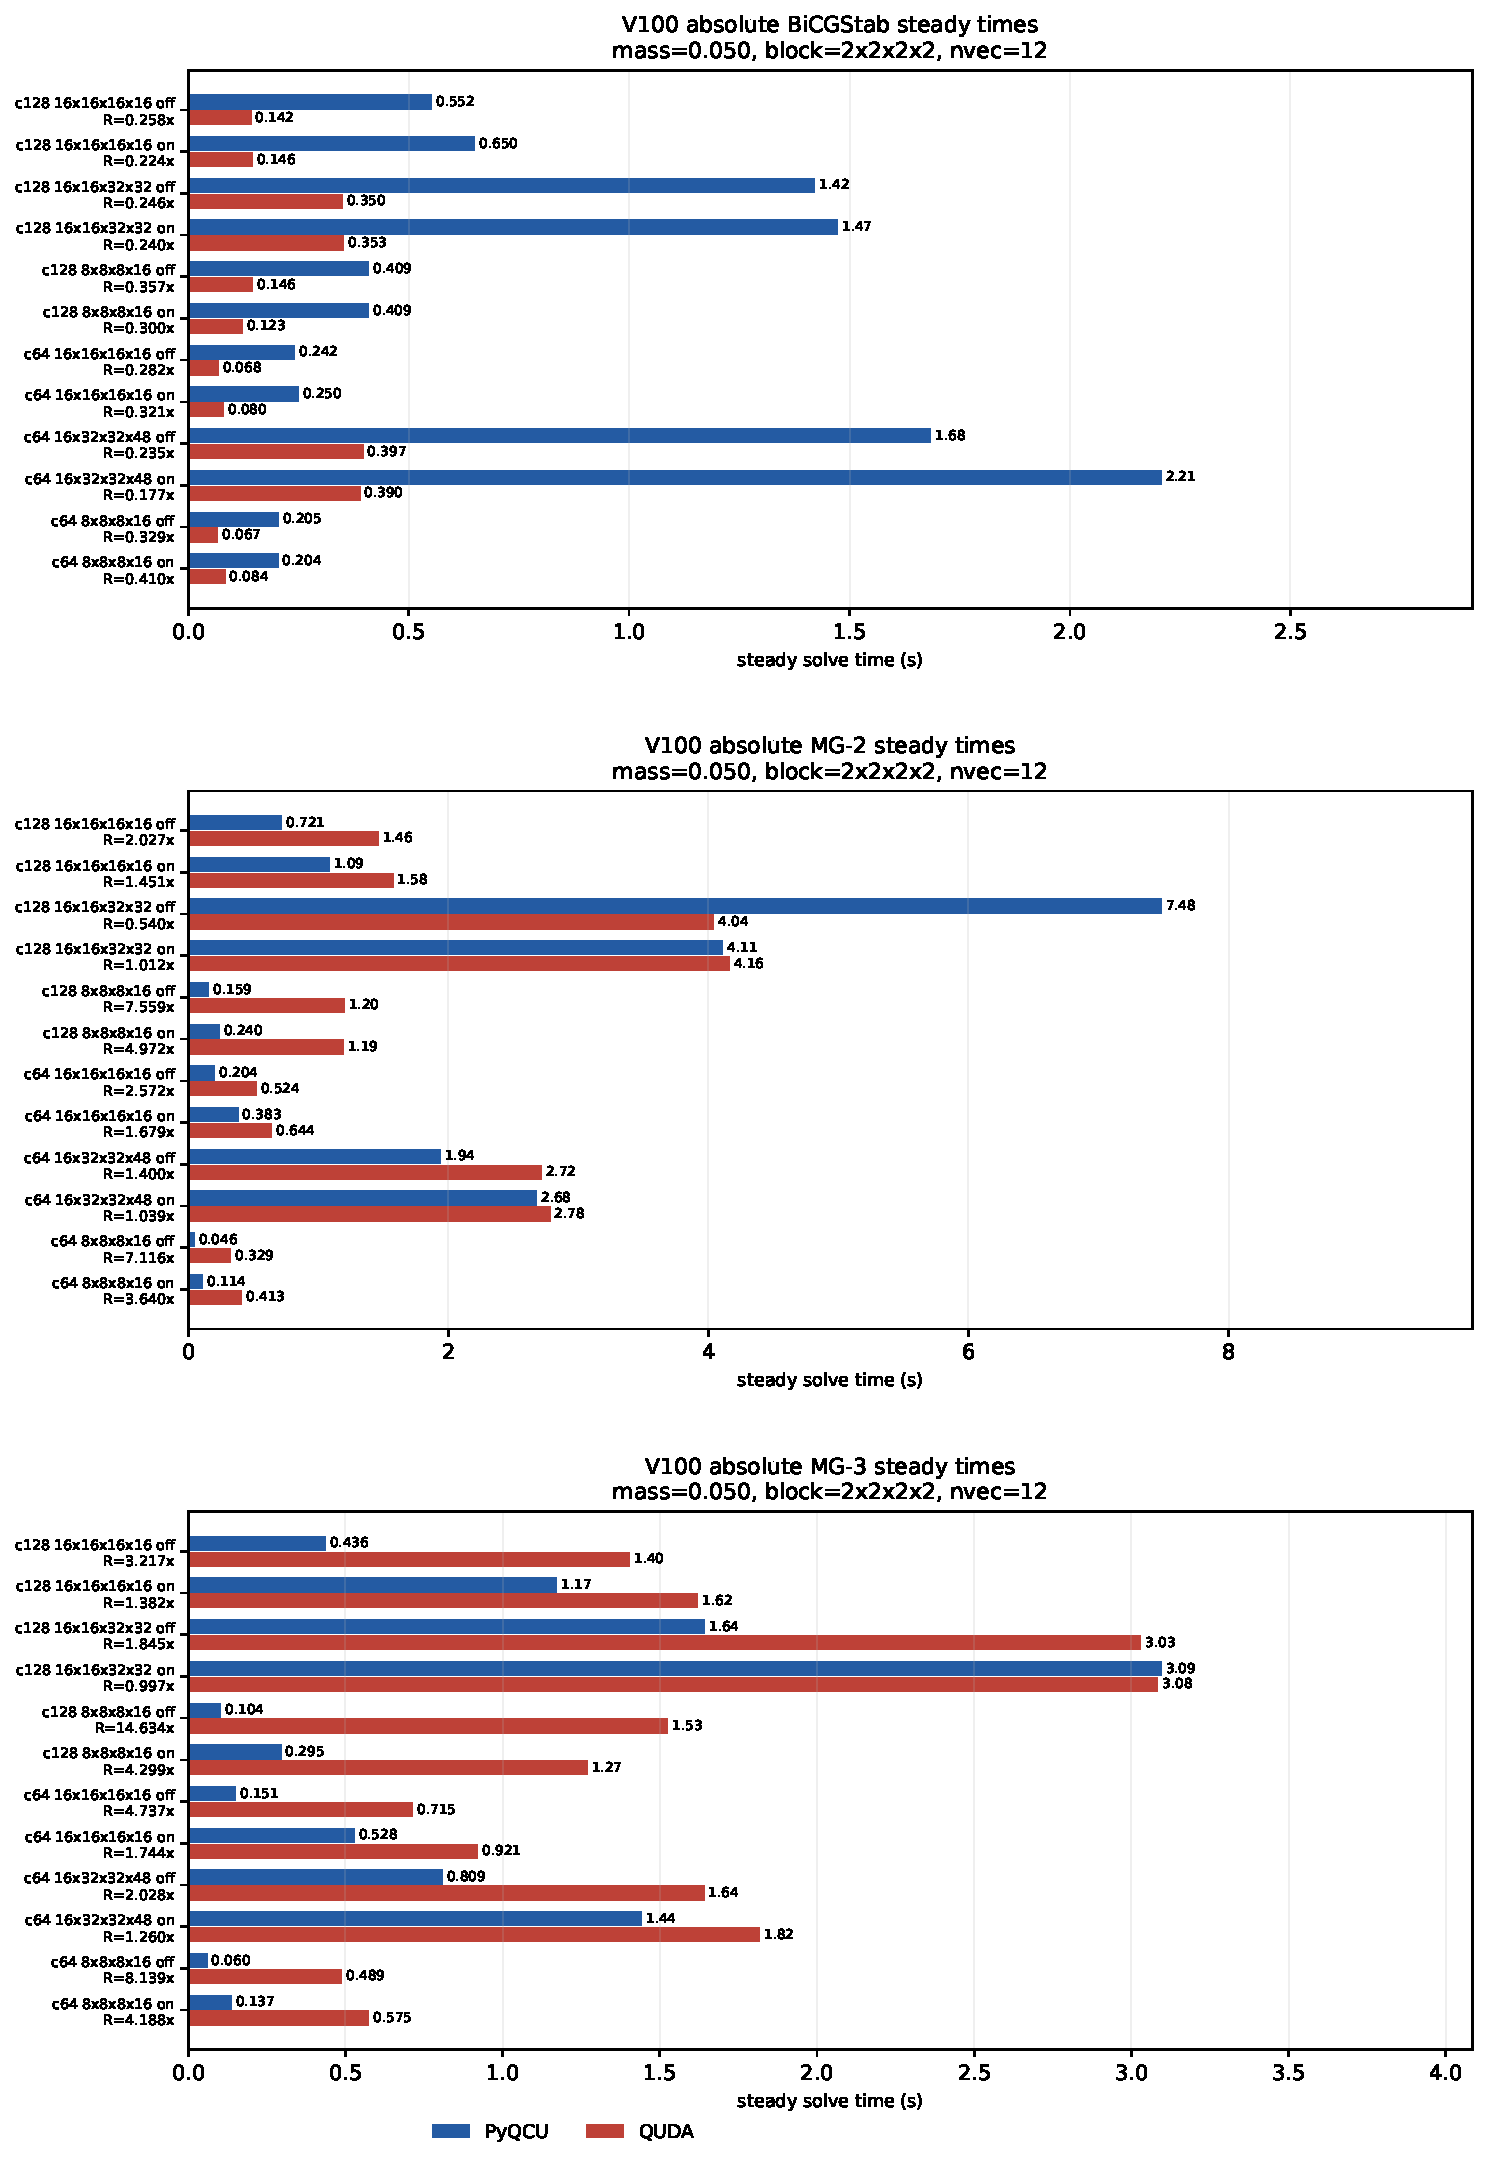
\includegraphics[width=0.98\linewidth,height=0.84\textheight,keepaspectratio]{mg_absolute_times_v100.pdf}
\caption{V100 的 BiCGStab、MG-2、MG-3 绝对 steady 耗时。}
\end{figure}

\begin{figure}[p]
\ContinuedFloat
\centering
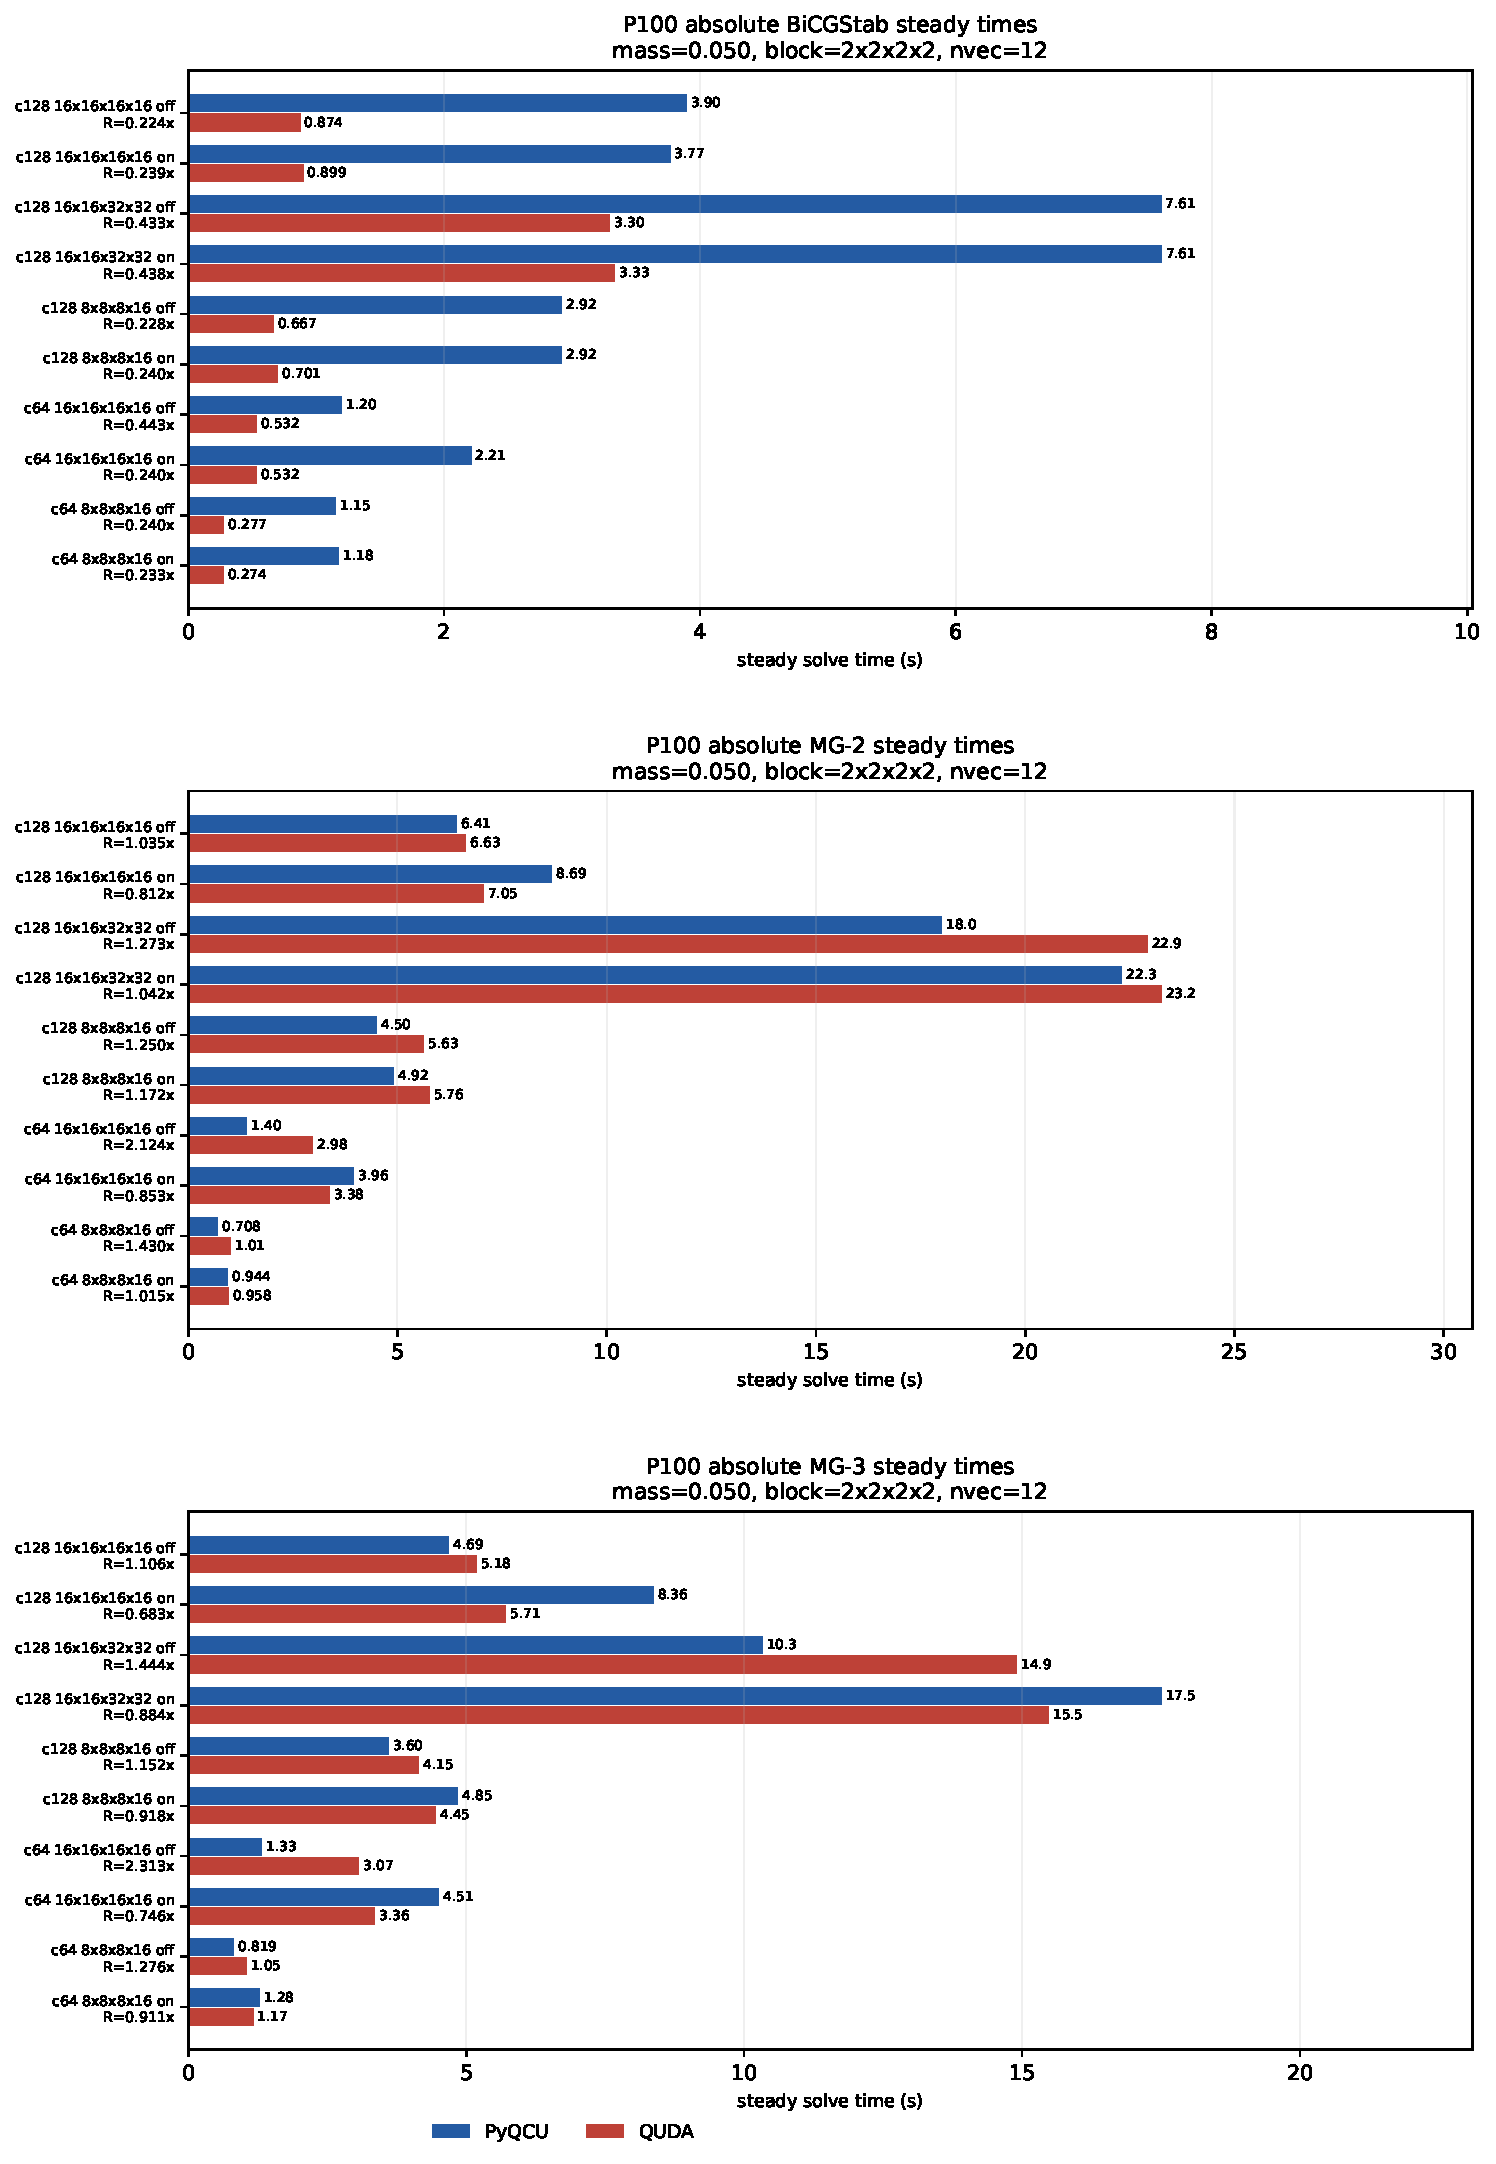
\includegraphics[width=0.98\linewidth,height=0.84\textheight,keepaspectratio]{mg_absolute_times_p100.pdf}
\caption{（续）P100 绝对 steady 耗时。}
\end{figure}

\begin{figure}[p]
\centering
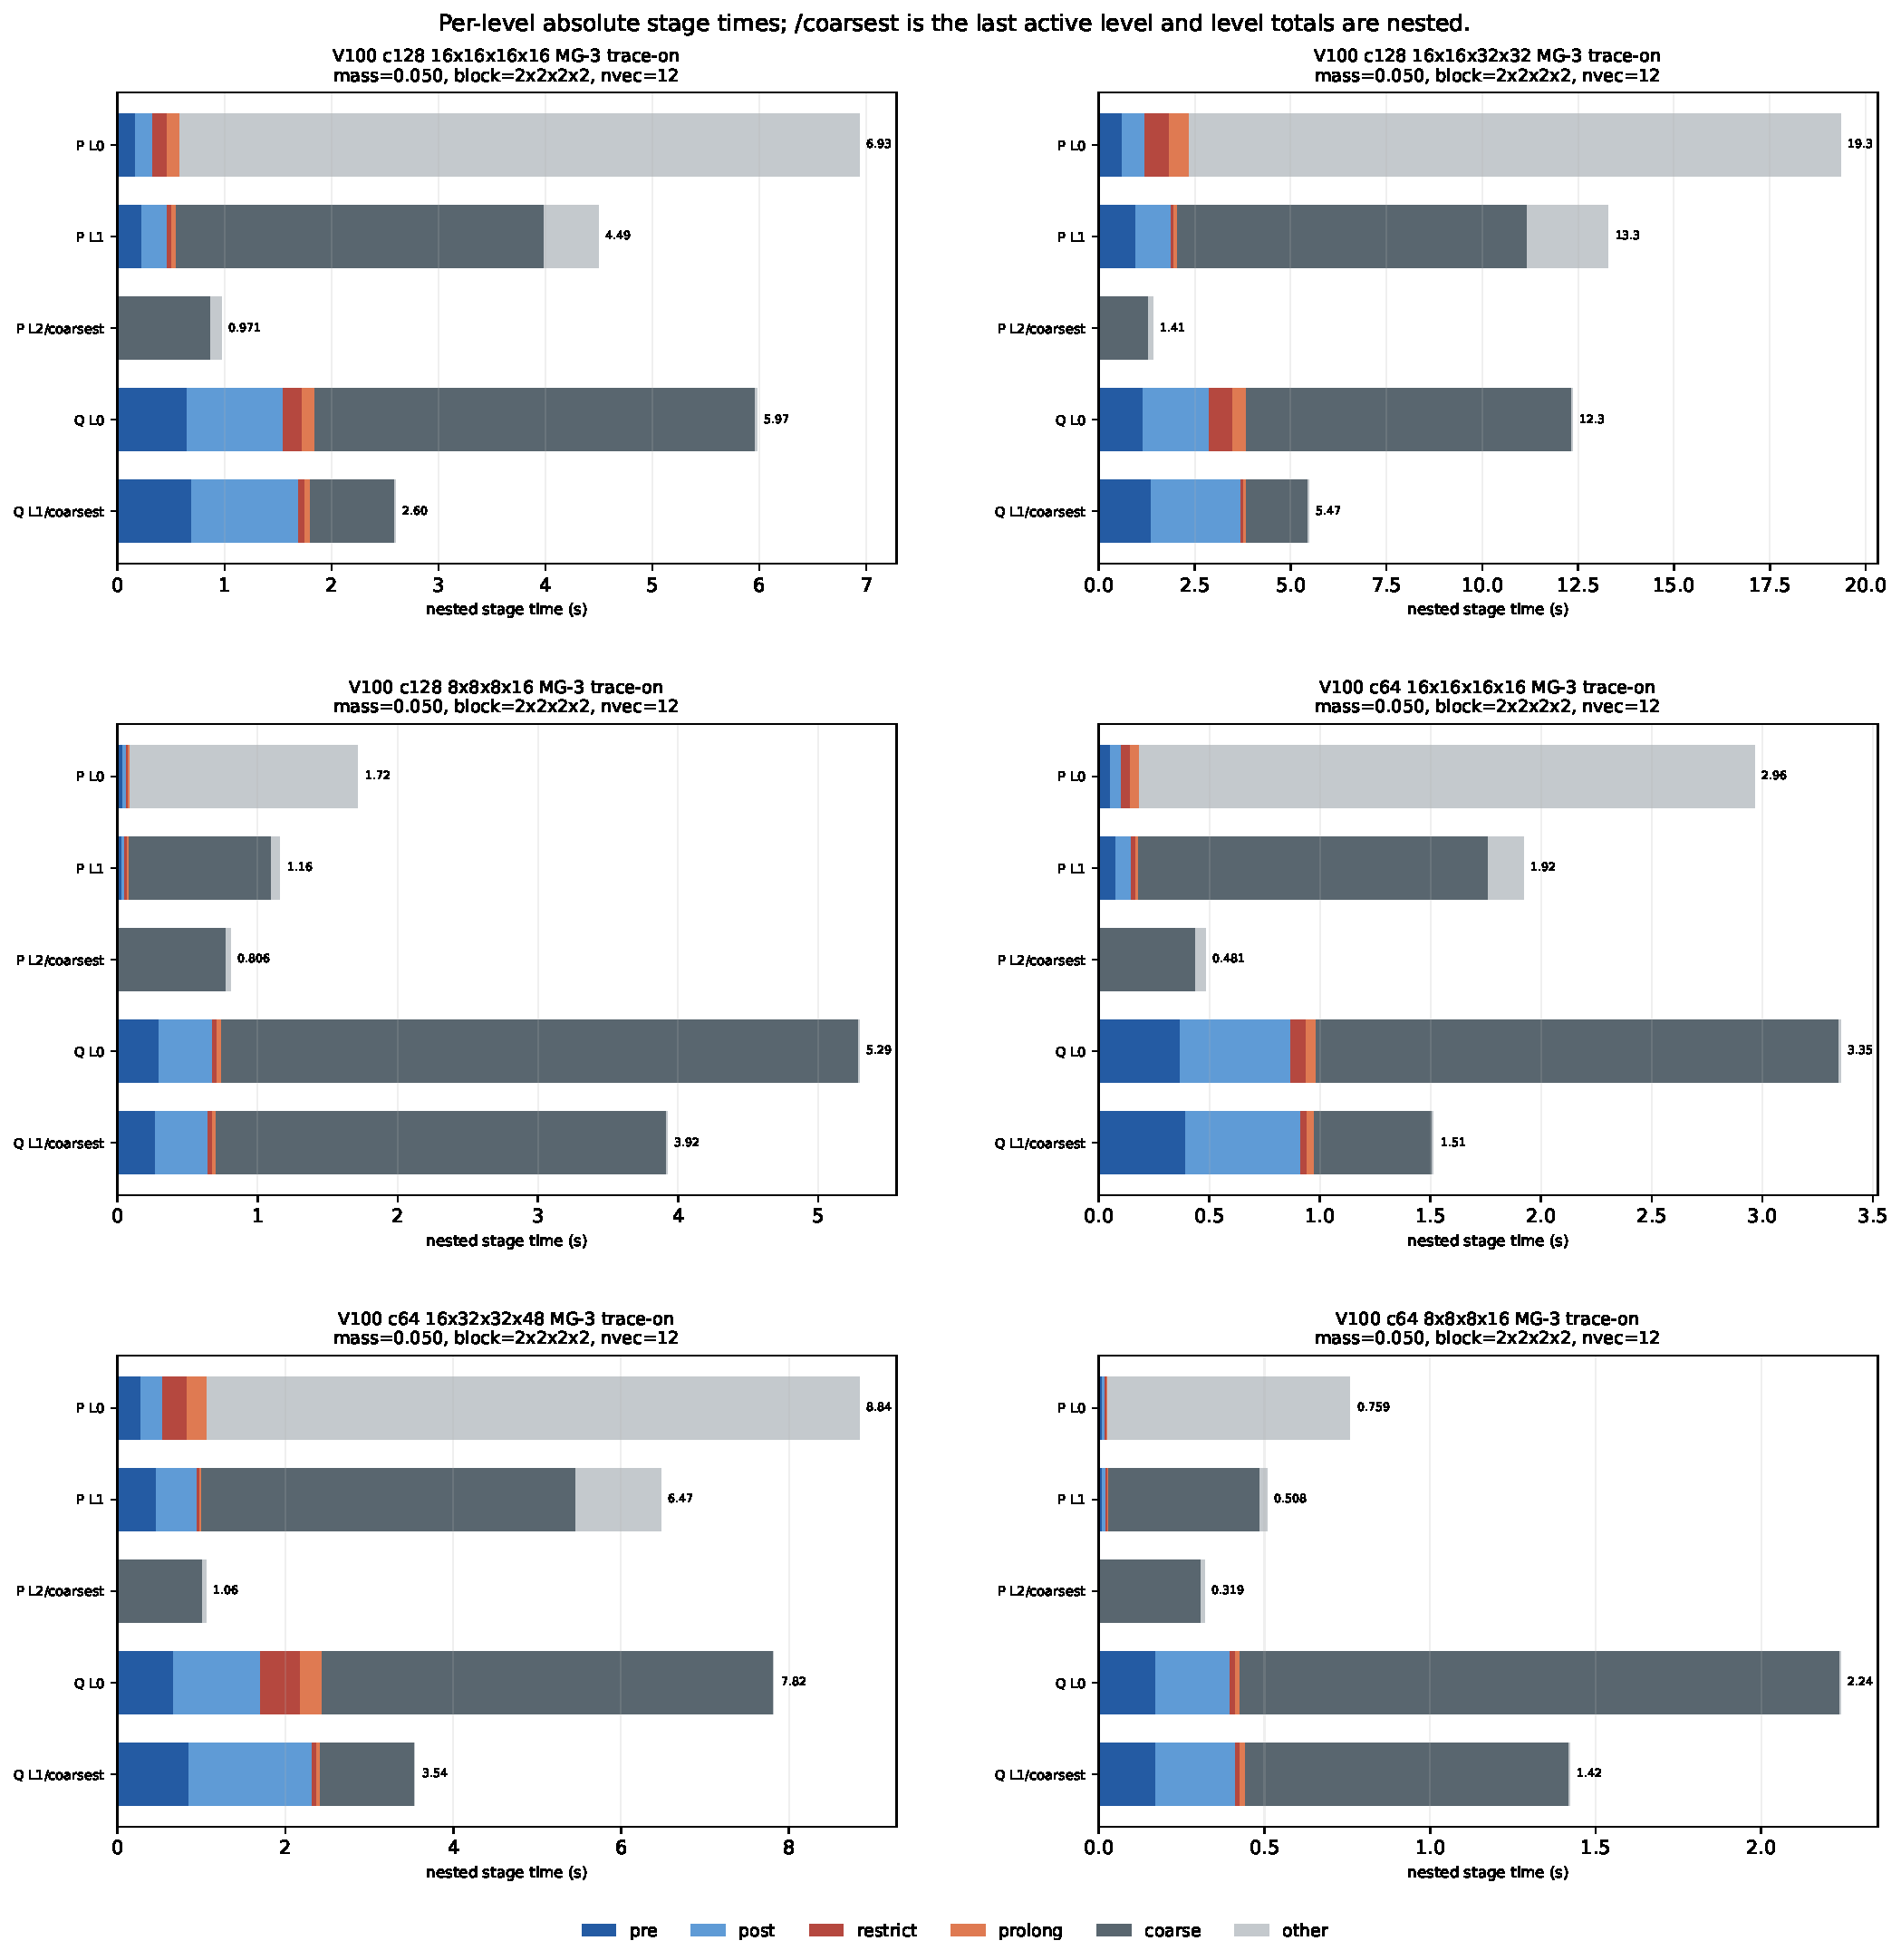
\includegraphics[width=0.98\linewidth,height=0.84\textheight,keepaspectratio]{mg_stage_linear_v100_mg3.pdf}
\caption{V100 MG-3 的逐层阶段耗时，用于观察最粗层量级；两侧阶段边界
不完全同构，不能把同名阶段逐个等同。}
\end{figure}

\begin{figure}[p]
\centering
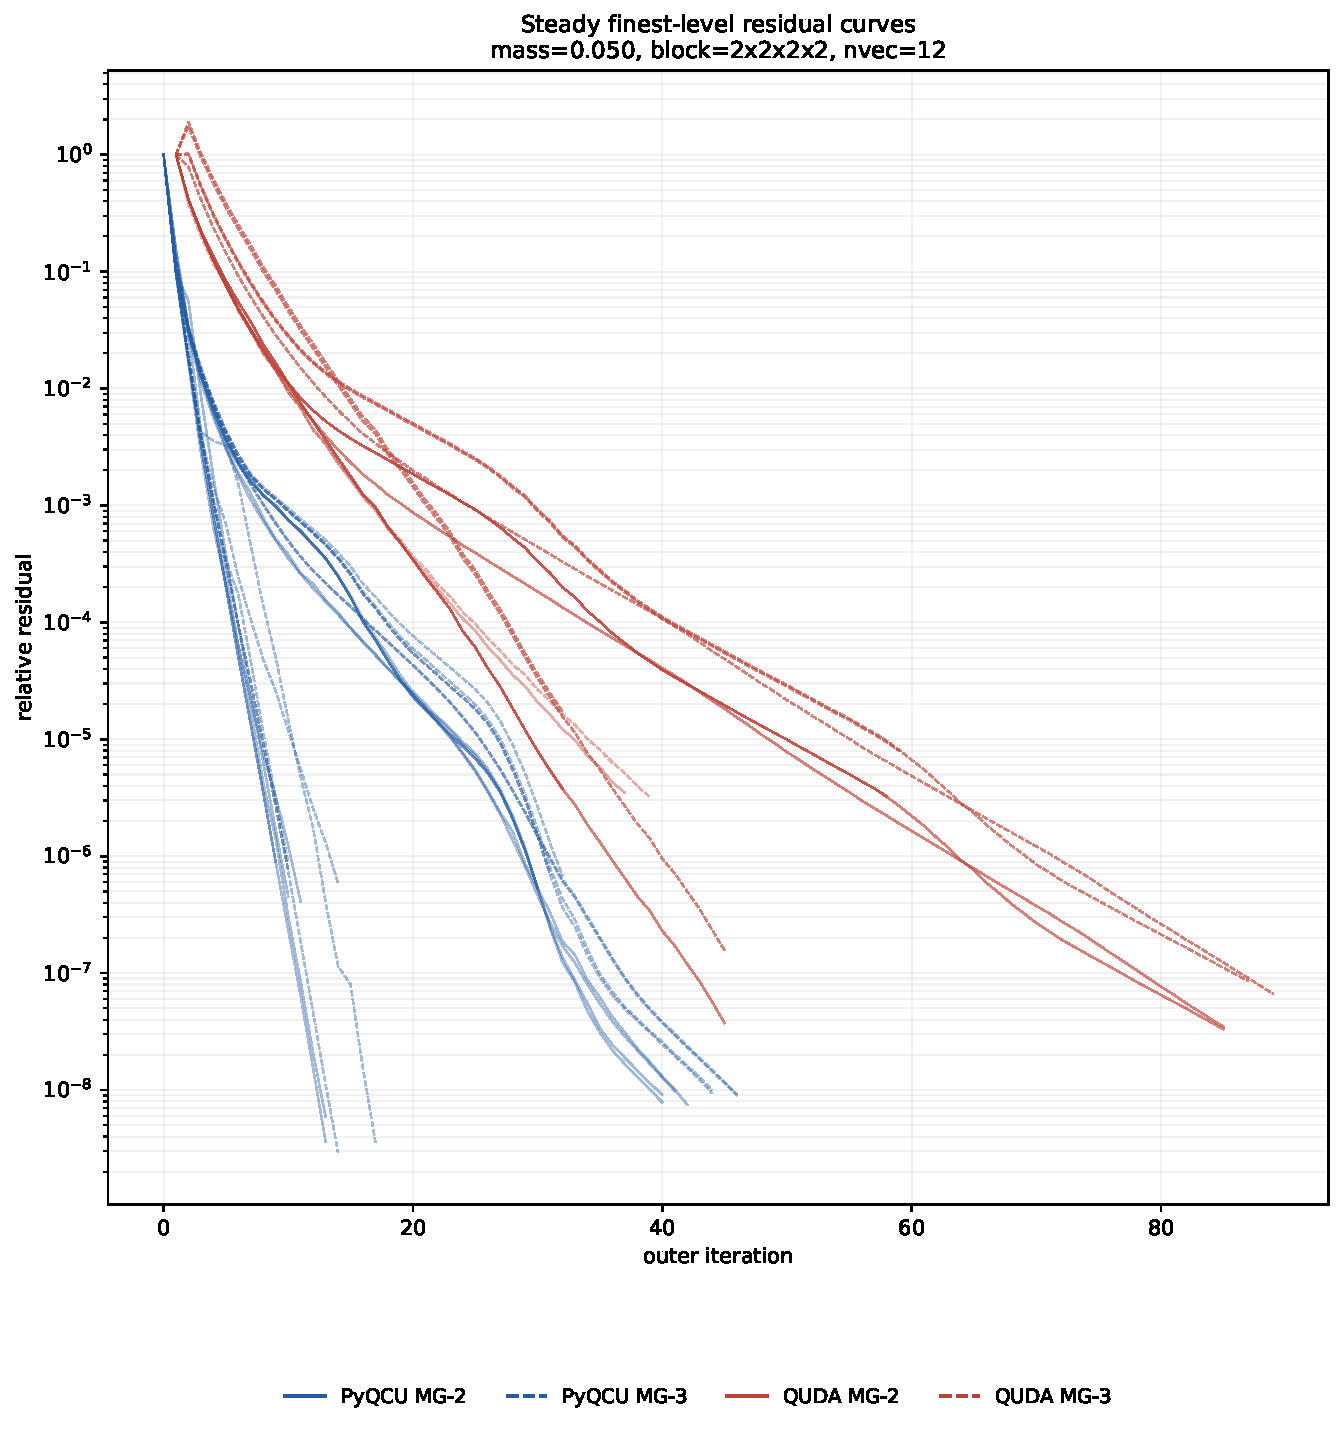
\includegraphics[width=0.94\linewidth,height=0.82\textheight,keepaspectratio]{mg_finest_residual_linear.pdf}
\caption{最细层相对残差总览。PyQCU 与 QUDA 的递推 residual scalar
定义不同，最终通过与否只由独立 full-operator true residual 判定。}
\end{figure}

\clearpage
\section{最终检查清单}

\begin{enumerate}[leftmargin=2em]
  \item 原始 test27 数据未改写：新生成器只读 combined JSON，输出新目录。
  \item 所有派生数字来自公开字段或代数重排；没有手工替换实验值。
  \item PyQCU/QUDA 的算法组合分别列出，且明确 test27 中 QUDA 禁用 MMA。
  \item 全局优势与 MG 优势分栏，BiCGStab 反例保留。
  \item 每个优化建议都有验收门或标注为候选。
  \item 架构图与性能图均有数据或源码边界说明。
\end{enumerate}

\end{document}
